\documentclass[10pt]{beamer}
\usetheme{Boadilla} % My favorite!
\setbeamercovered{invisible}
% To remove the navigation symbols from 
% the bottom of slides%
\setbeamertemplate{navigation symbols}{} 
\setbeamertemplate{itemize items}[default]
\setbeamertemplate{enumerate items}[default]
\xdefinecolor{lavendar}{rgb}{0.2, 0.2, 0.72}
%
\usepackage{graphicx,epsfig}
\usepackage{tikz}

%\usepackage{bm}         % For typesetting bold math (not \mathbold)
%\logo{\includegraphics[height=0.6cm]{yourlogo.eps}}
%

\newcommand{\be}{\begin{equation*}}
\newcommand{\ee}{\end{equation*}}
\newcommand{\ba}{\begin{eqnarray}}
\newcommand{\ea}{\end{eqnarray}}

\newcommand{\vso}{\vskip15pt}
\newcommand{\vst}{\vskip30pt}



\usepackage{tikz}
\usetikzlibrary{shapes,arrows,positioning}

\tikzstyle{decision} = [diamond, draw, fill=blue!20, text width=4.5em, text badly centered, inner sep=0pt]
\tikzstyle{block} = [rectangle, draw, fill=blue!20, text width=5em, text centered, rounded corners,
 minimum width=3.5cm]
\tikzstyle{line} = [draw, -latex]


\def\smallfrac#1#2{\hbox{${{#1}\over {#2}}$}}


\AtBeginSection[]
{
  \begin{frame}<beamer>{}
  \frametitle{Outline}
    \tableofcontents[currentsection]
  \end{frame}

}
\title[]{Parton Distributions with LHC Data}
\author{Nathan Hartland}
\institute
{
University of Edinburgh\\
%\includegraphics[height=2cm]{edinburghcrest.pdf}
\medskip
}
% \today will show current date. 
% Alternatively, you can specify a date.
%
\titlegraphic{\includegraphics[height=2cm]{edinburghcrest.pdf}}

\date{\today}


\begin{document}
\renewcommand{\inserttotalframenumber}{36}


\begin{frame}
\begin{centering}
\vskip20pt
\center{\huge\color{lavendar} \textbf{Parton Distributions with LHC Data}}
\vskip20pt
Nathan Hartland\\

\small{University of Edinburgh}\\
\vso
\includegraphics[height=2cm]{edinburghcrest.pdf}

\vskip10pt
{\bf The NNPDF Collaboration:}\\
R.~D.~Ball, V.~Bertone, S.~Carrazza,\\ F.~Cerutti,
C.~Deans, L.~Del~Debbio, S.~Forte, N.H\\
A.~Guffanti, J.I.~Latorre, J.~Rojo and M.~Ubiali. 
\vskip20pt
HEP phenomenology joint Cavendish-DAMTP seminar
University of Cambridge\\
Thursday 29th November 2012

\end{centering}

\end{frame}

\begin{frame}
\frametitle{What is a parton distribution function?}
\small \underline{QCD Factorisation:} \\
When considering a scattering process with a single hadron in the initial state, the calculation may be factorized into a soft part and a perturbatively calculable hard part.
\be \sigma_X(Q^2)= \sum_{a} \int_0^1 dx\; f_a(x,\mu^2)\sigma_{q_a \to X} \left( x,\frac{Q^2}{\mu^2} \right) \ee

\begin{columns}
\begin{column}{0.5\textwidth}
\includegraphics[width=\textwidth]{DIS.eps}
\end{column}

	\begin{column}{0.5\textwidth}
	\begin{block}{\small $\sigma_{q_a \to X} $ - perturbative}
	\footnotesize Hard cross section for lepton scattering off a parton of flavour $a$, carrying a fraction $x$ of the parent hadron's momentum.
	\end{block}
	
	\begin{block}{\small $f_a(x,\mu^2) $ - non-perturbative}
		\footnotesize Parton distribution function describing nonperturbative dynamics of target hadron. At LO can be interpreted as the probability of finding a parton of flavour
		$a$ with momentum fraction $x$ inside the target hadron.
	\end{block}

	\end{column}
\end{columns}
\end{frame}

\begin{frame}
\frametitle{Parton distributions - what's on the market?}

\begin{itemize}
\item Many different determinations of parton distributions are available.
\end{itemize}

\begin{columns}
	\begin{column}{0.5\textwidth}
		\includegraphics[width=\textwidth]{pdf_xSigma_log_band_comparison_others.eps}
	\end{column}

	\begin{column}{0.5\textwidth}
		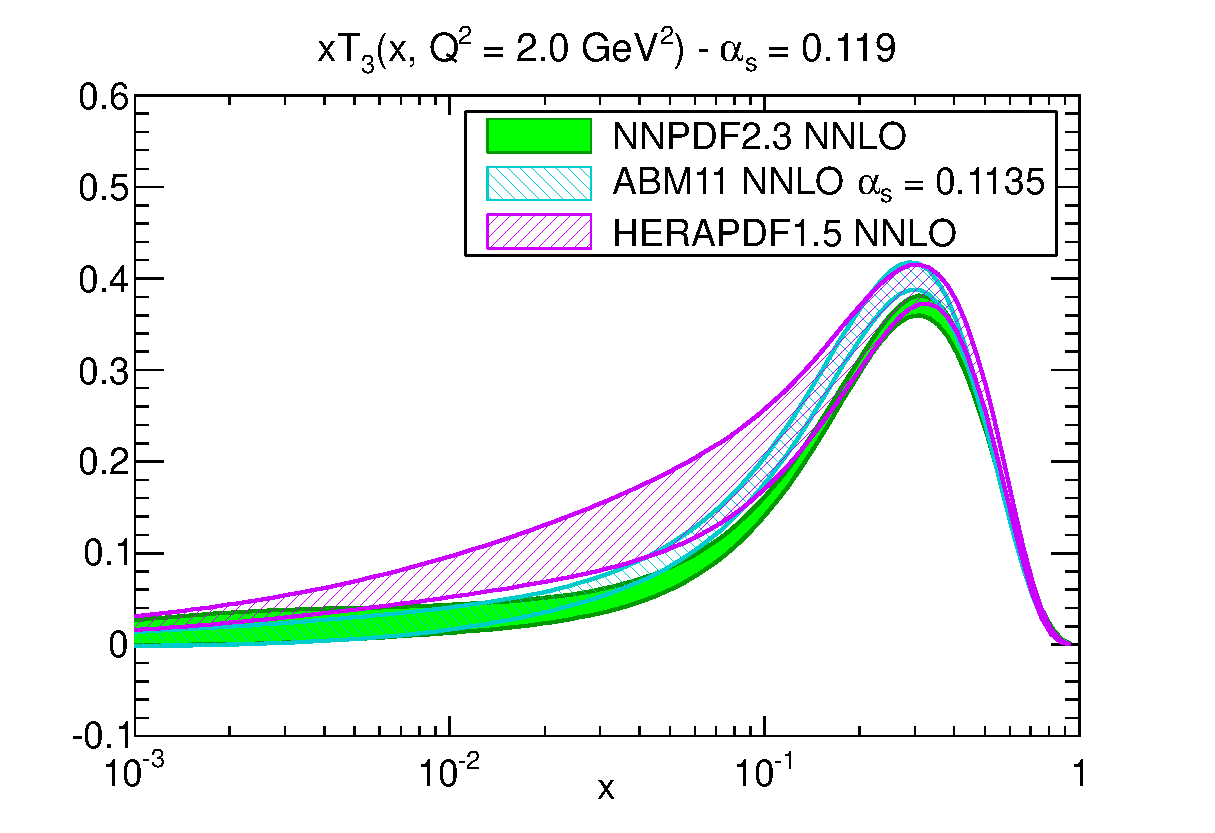
\includegraphics[width=\textwidth]{pdf_xT3_log_band_comparison_others_b.eps}
	\end{column}
\end{columns}

\begin{columns}
	\begin{column}{0.5\textwidth}
		\footnotesize{\be \Sigma(x) = \sum_q q(x)+\bar{q}(x) \ee}
	\end{column}

	\begin{column}{0.5\textwidth}
		\footnotesize{
\begin{eqnarray}
\nonumber T_3(x)&=&u_V(x) - d_V(x). \\
\nonumber  &=&\left( u(x) - \bar{u}(x)\right) - (d(x) - \bar{d}(x))
\end{eqnarray}
}

	\end{column}
\end{columns}


\centering{\underline{Collaborations:} $\quad$MSTW, CTEQ, NNPDF, HERAPDF, ABM, GJR}


\end{frame}

\begin{frame}
\frametitle{How can we determine proton PDFs?}

\begin{columns}
\begin{column}{0.6\textwidth}
\begin{enumerate}
\item<1-> Theoretical input
\begin{itemize}
\item (N)NLO QCD, $\alpha_S$, HQ Treatment
\end{itemize}
\vskip15pt
\item<1-> PDF Parameterization
\begin{itemize}
\item What is a suitable choice of functional form?
\end{itemize}
\vskip15pt

\item<1-> Theoretical predictions
\begin{itemize}
\item How can we make fast pQCD predictions for experimental data while including higher order corrections?
\end{itemize}
\vskip15pt

\item<1-> Comparison to data
\begin{itemize}
\item What does the (LHC) data tell us about proton structure?
\end{itemize}
\end{enumerate}
\end{column}
\begin{column}{0.3\textwidth}

\scalebox{0.6}{
      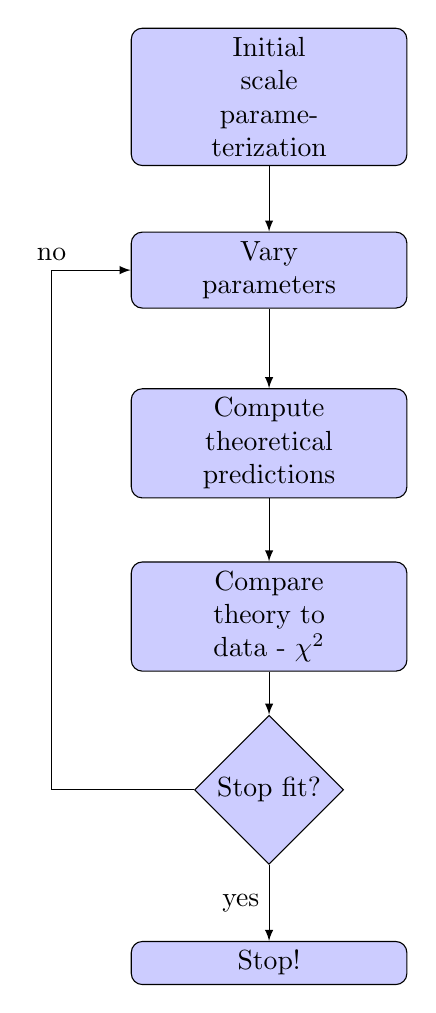
\begin{tikzpicture}[node distance=2.2cm]
        \node[block]                  (init){Initial scale parameterization};
        \node[block, below of=init]   (nbrh){Vary parameters};
        \node[block, below of=nbrh](ovgt){Compute theoretical predictions};
        \node[block, below of=ovgt]   (accp){Compare theory to data - $\chi^2$};
        \node[decision, below of=accp]   (stop){Stop fit?};
         \node[block, below of=stop]   (stopfit){Stop!};

        % invisible node helpful later
        \node[left=1cm of ovgt,scale=0.05](inv){};

        \path[line] (init) --          (nbrh);
        \path[line] (nbrh) --          (ovgt);
         \path[line] (ovgt) --          (accp);
          \path[line] (accp) --          (stop);
          
        \path[line] (stop) -- node[left]{yes}(stopfit);

       \path[-,draw] (stop) -| node{} (inv.north);
       \path[line]{} (inv.north) |- node[above]{no} (nbrh);    
           
      \end{tikzpicture}%
      }
      
      \end{column}
      
      
 \end{columns}
      \vskip10pt
\centering{In this talk $\to$ $ \chi^2[f] = \frac{1}{N_{\mathrm{dat}}}\sum_{i,j}^{N_{\mathrm{dat}}} \left( D_i - T_i[f] \right) \sigma_{ij}^{-1}  \left( D_j - T_j[f] \right)$.}



\end{frame}

\begin{frame}
\frametitle{What do we know from theory?}
\small \underline{Factorisation scale dependance:} \\
PDFs evolve with scale according to the DGLAP equations.
\be \mu^2 \frac{\partial f(x,\mu^2)}{\partial \mu^2} = \int_x^1 \frac{dy}{y} P\left( \frac{x}{y} \right) f (y,\mu^2)  \ee
Where $P$ are the perturbatively calculable splitting functions.

\small \underline{Theoretical constraints:} \\
\begin{itemize}
\item PDF Sum Rules
\be \int_0^1 dx\; x(\Sigma(x) + g(x)) = 1,\quad\quad   \sum_{q} \int_0^1 dx\; (q(x)-\bar{q}(x)) = 3 \ee
\end{itemize}

\begin{itemize}
\item Approx asymptotic behaviour
\be x \to 0: \quad f_V(x) \sim x^{-\alpha}\ee
\be x \to 1: \quad f_V(x) \sim (1-x)^{\beta}\ee
\end{itemize}

\begin{itemize}
\item Positivity of \emph{physical observables} ($F$, $\sigma$)
\begin{itemize}
\item Beyond LO pdfs are not restricted to be positive.
\end{itemize}
\end{itemize}

\begin{center}
Aside from these constraints,\\ $x$ dependence must be determined by fitting to experimental data!
\end{center}


\end{frame}


\begin{frame}
\frametitle{Parton distribution fitting - initial scale parameterization}
\begin{itemize}
\item PDFs at the initial scale are parametrized by some functional form
\end{itemize}

\begin{columns}
\begin{column}{0.5\textwidth}
\begin{block} {\centering \small Typical Parameterizations}
\begin{itemize}
\item<1-> \small MSTW08 $\sim$ 28 total PDF parameters 
\end{itemize}
    \be f_v(x) \sim ax^{b}(1-x)^{c}(1+d\sqrt{x}+e x),\ee   \begin{itemize}
\item<1-> \small CT10   $\sim$ 26 total PDF parameters 
	\end{itemize}
	\small \be f_v(x) \sim ax^b(1-x)^c \exp{(dx + ex^2 + f\sqrt{x})}.\ee \begin{itemize}
\item<1-> \small HERAPDF   $\sim$ 10 total PDF parameters 
	\end{itemize}
		\small \be f_v(x) \sim ax^b(1-x)^c \exp{(1+dx + ex^2)}.\ee

\end{block}

\begin{block}
{ \small \centering NNPDF functional form}
\begin{itemize}
\item<1-> \small NNPDF $\sim$ 259 total PDF parameters 
\end{itemize}
\be f(x) \sim ax^b(1-x)^{c} \mathrm{NN}(x). \ee
\end{block}
\end{column}
	\begin{column}{0.4\textwidth}
	\small 
	
\begin{itemize} \small
\item<1-> Attempt to minimise figure of merit by varying ($a$..$f$).
\item<1-> Choice of functional form: Parameterization \emph{bias}
\end{itemize}
\vskip10pt
\begin{center}
\underline{NNPDF Strategy}\end{center}
\vskip-10pt
\begin{itemize} \small
\item<1-> Minimise bias by choosing extremely flexible functional form
\item<1-> Each PDF parametrized by a 2-5-3-1 Neural Network
\item<1-> 259 Free parameters $\to$ \textbf{massively redundant} parameterization
\item<1-> $b,c$  $\to$ randomised preprocessing.

\end{itemize}

\end{column}
\end{columns}
\end{frame}


\begin{frame}
\frametitle{Theoretical Predictions}
Calculate theoretical predictions for comparison with experimental data.\\
Evolve to required scale and perform convolution with hard coefficients.\\
\vskip10pt
\underline{DIS data:} cross sections parametrized in terms of  \textbf{structure functions}:
\be F_i(x,Q^2) = \int\frac{dy}{y} C_{i}^{j}(y,\alpha_s(Q^2))f_j\left(\frac{x}{y},Q^2\right) \ee

\underline{Hadron Collider data:} perform double convolution over PDFs
\be \sigma_X= \sum_{a,b} \int_0^1 dx_1dx_2 f_a(x_1,Q^2)f_b(x_2,Q^2)\sigma_{q_aq_b \to X} \left( x_1,x_2,Q^2 \right) \ee
Hadronic data dependant upon PDFs through parton-parton luminosities:
\be \Phi_{ij}(\tau,M_X^2) = \frac{1}{s}\int_\tau^1\frac{dx_1}{x_1} f_i(x_1,M_X^2)f_j(\tau/x_1,M_X^2) \ee

\end{frame}


\begin{frame}
\small
\frametitle{Minimisation and Stopping in NNPDF}
\textbf{Minimisation by genetic algorithms}\\
\underline{Problem}: Very large parameter space, $\chi2$ highly nonlocal. \begin{itemize}
\item<1-> Minimisation is challenging.
\end{itemize}\underline{Solution}: Genetic Algorithms (GA)
\begin{itemize}
\item<1-> Generate mutations of fit parameters.
\item<1-> Select those mutations that minimise figure of merit.
\end{itemize}
\vskip10pt
\textbf{ Dynamical fit stopping by cross-validation}\\
\underline{Problem}:  extremely flexible parameterisations are prone to \emph{overfitting}.
\\
\begin{itemize}
\item<1->Fit has so many parameters, the minimum $\chi^2$ corresponds to a fit not only to
the data, but also statistical noise.
\end{itemize}
\underline{Solution}:  dynamical stopping by \emph{Cross Validation}.
\begin{itemize}
\item<1-> Split the dataset into a training set and a validation set.
\item<1-> Use the training set for minimisation, monitor the $\chi^2$ to the validation set.
\item<1-> Stop the fit when the $\chi^2$ to the validation set starts to increase while
the $\chi^2$ to training set is still decreasing.

\end{itemize}
\end{frame}


\begin{frame}
\frametitle{Cross Validation}
 \begin{figure}[b!]
    \begin{center}
      \includegraphics[width=0.9\textwidth]{chi2ite-1004-NMC-pd.eps}
    \end{center}
\end{figure}
\end{frame}


\begin{frame}
\frametitle{Parton distribution fitting - Datasets}

\begin{itemize}
\item<1-> \small PDF determination datasets divided into global and restricted determinations.
\end{itemize}

\begin{columns}

\begin{column}{0.3\textwidth}

\begin{table}
\tiny
\begin{tabular}{c|c}
\multicolumn{2}{c}{\bf PDF Fit Datasets}  \\
\hline 
  Fit & Dataset   \\
\hline 
MSTW08 & \textbf{global}  \\
CT10 & \textbf{global}  \\
NNPDF2.1 & \textbf{global}  \\
HERAPDF1.5 & HERA DIS \\
ABM11 & DIS+DY \\

\hline
\end{tabular}
\end{table}

\begin{table}
\tiny
\begin{tabular}{c|c}
\multicolumn{2}{c}{\bf NNPDF2.1 NNLO Dataset}  \\
\hline 
  Experiment & Datapoints   \\
\hline 
DIS (Fixed Target) & 1952  \\
DIS (HERA) & 834  \\
Fixed Target DY & 318  \\
Tevatron W\/Z & 70 \\
Tevatron Jets & 186 \\
\hline
Total   & 3360 \\

\hline
\end{tabular}
\end{table}


\end{column}

\begin{column}{0.7\textwidth}
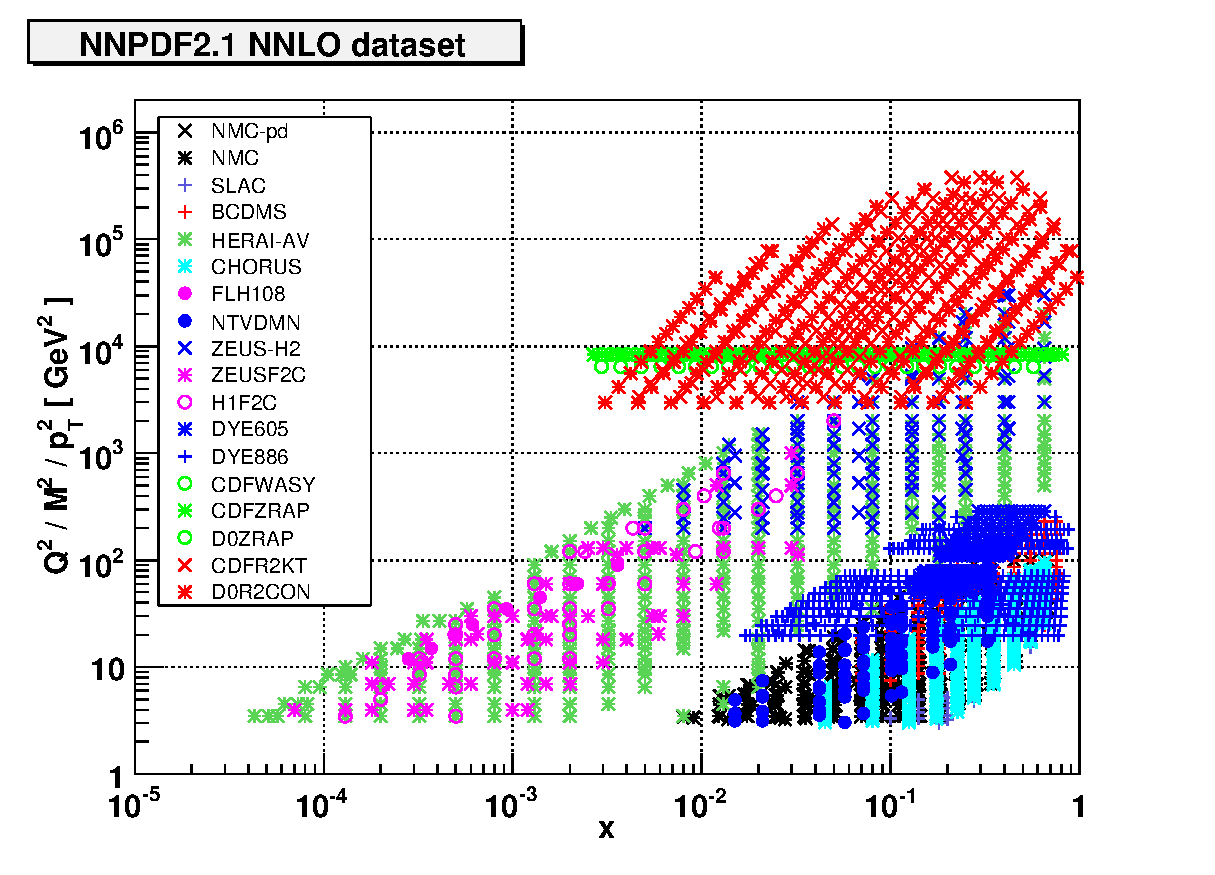
\includegraphics[width=\textwidth]{kin21nnlo.eps}
\end{column}


\end{columns}


\center{\underline{Reliable propagation of experimental error is crucial}}

\end{frame}


\begin{frame}
\frametitle{Standard approach to parton fitting - uncertainties}
How to propagate uncertainties from the experimental data to the PDFs?
\underline{Standard Approach}: Linear propagation of uncertainties by Hessian Method.
\begin{itemize}
		\item<1->For a set of fit parameters $\{ a\} $ define a tolerance in $\chi^2$:
		\be \Delta\chi^2(a) \equiv \chi^2(a) - \chi^2(a^\mathrm{min}) = \sum^n_{i,j=1}H_{ij}(a_i-a_i^\mathrm{min})(a_j - a_j^\mathrm{min}). \ee
		\item<1-> Determine PDFs on surface of constant $\Delta\chi^2=T$ in parameter space.
		\begin{itemize}
			\item<1-> Numerical difficulties: Need to use rescaled eigenvectors of $H$.
		\end{itemize}
		\item<1-> Obtain $2n$ PDF sets $S_i^\pm$, where $n$ is the number of free parameters in the fit. \vso
		\item<1-> Uncertainty in an observable $\mathcal{O}$ given by:
		\be \mathrm{Var}[\mathcal{O}] = \frac{1}{2}\sum_{i=0}^n (\mathcal{O}[S_i^+] - \mathcal{O}[S_i^-] )^2.\ee
\end{itemize}

\end{frame}


\begin{frame}
\frametitle{Monte Carlo uncertainty determination}
\begin{itemize}
\item<1->Form an ensemble of $N$ artificial data 'replicas' by importance sampling the original data set.
\\
\item<1->The ensemble of artificial data replicas forms a representation of the probability distribution in data.
\\
\item<1->Perform a separate fit to each data replica, obtain an ensemble of PDF replicas.
\\
\end{itemize}
 \begin{figure}[b!]
    \begin{center}
      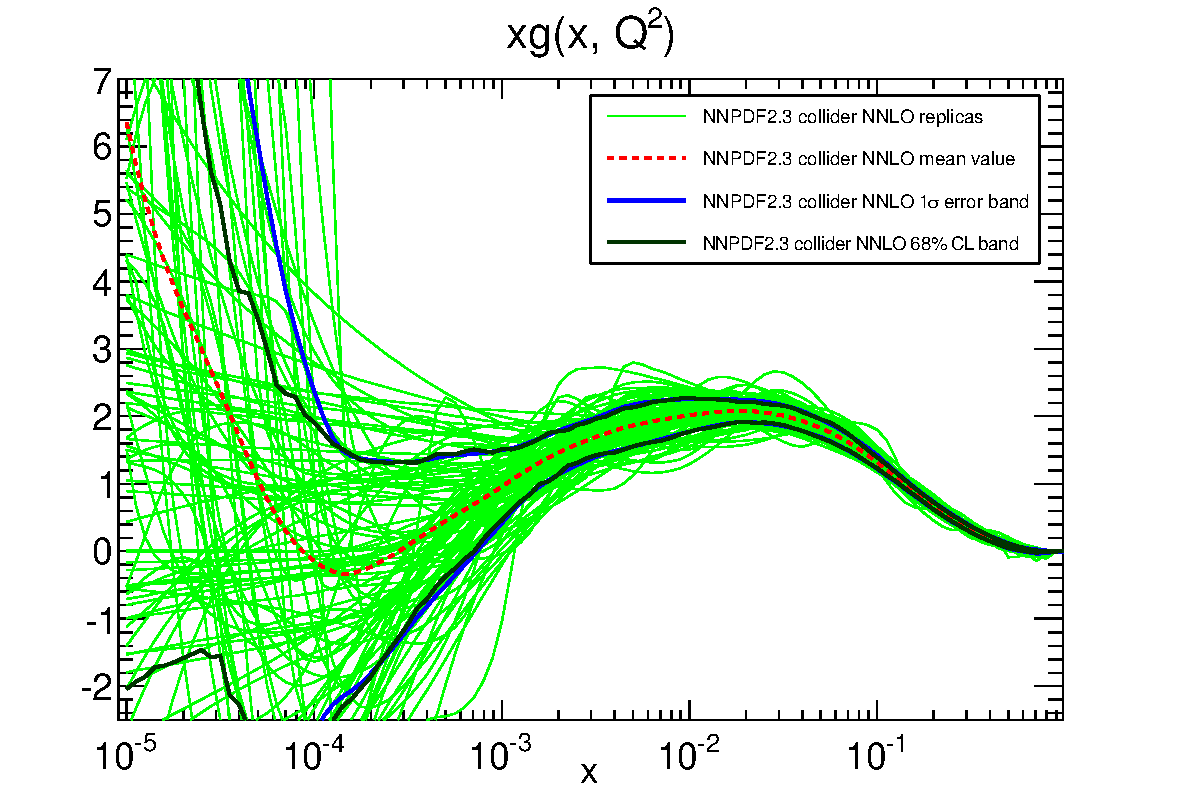
\includegraphics[width=0.45\textwidth]{xg_rep_Q_2_log-23coll-nnlo.pdf}
      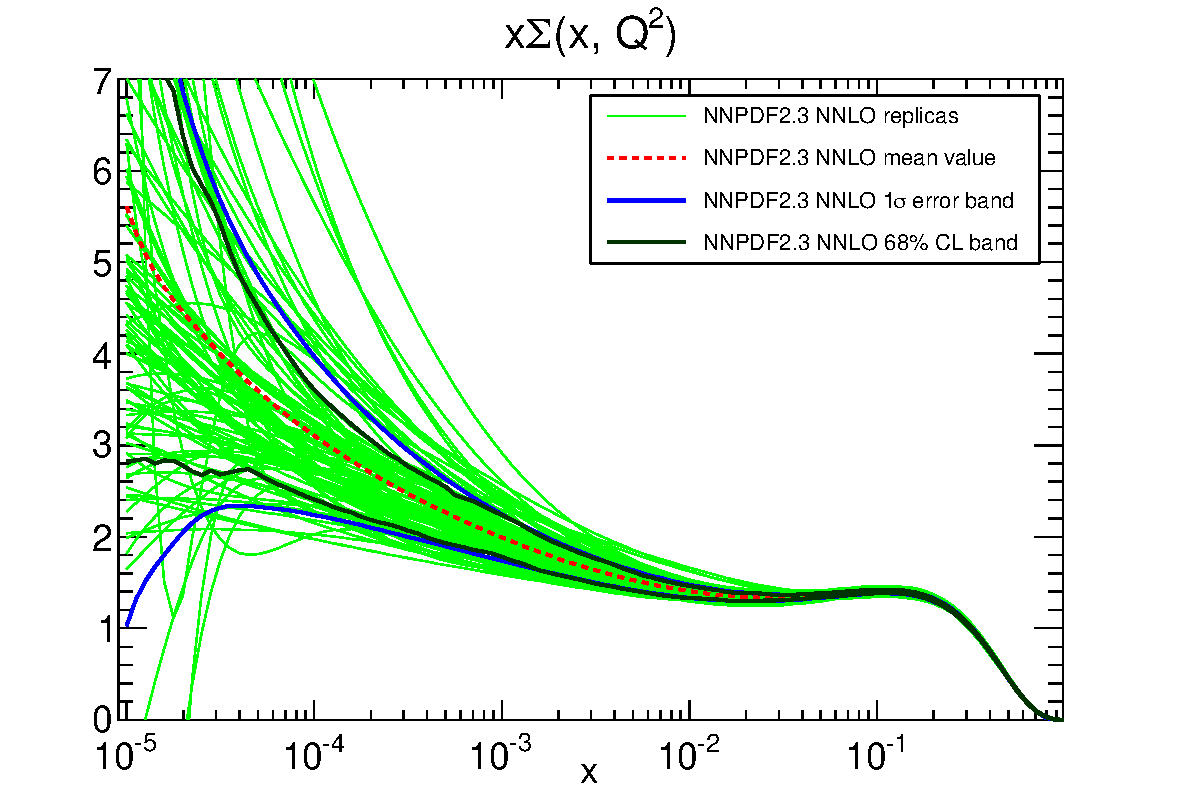
\includegraphics[width=0.45\textwidth]{xSinglet_rep_Q_2_log-23-nnlo.pdf}
    \end{center}
    \vskip-0.5cm
    \label{fig:pdf-jets}
\end{figure}

\end{frame}

\begin{frame}
\frametitle{NNPDF User Guide}

\begin{columns}
\begin{column}{0.4\textwidth}
\small
\begin{block} 
{ \small Central value predictions}
		\small \be \langle\mathcal{O}\rangle=\smallfrac{1}{N}\,\sum_{k=1}^{N}\mathcal{O}[f_k]\, .\ee
\end{block}
\vskip5pt
\begin{block}
{\small Uncertainties }
	\small	\be {\mathrm{Var}}[\mathcal{O}]=\smallfrac{1}{N}\,\sum_{k=1}^{N}(\mathcal{O}[f_k] -  \langle\mathcal{O}\rangle )^2 .\ee
\end{block}
\end{column}

\begin{column}{0.6\textwidth}
      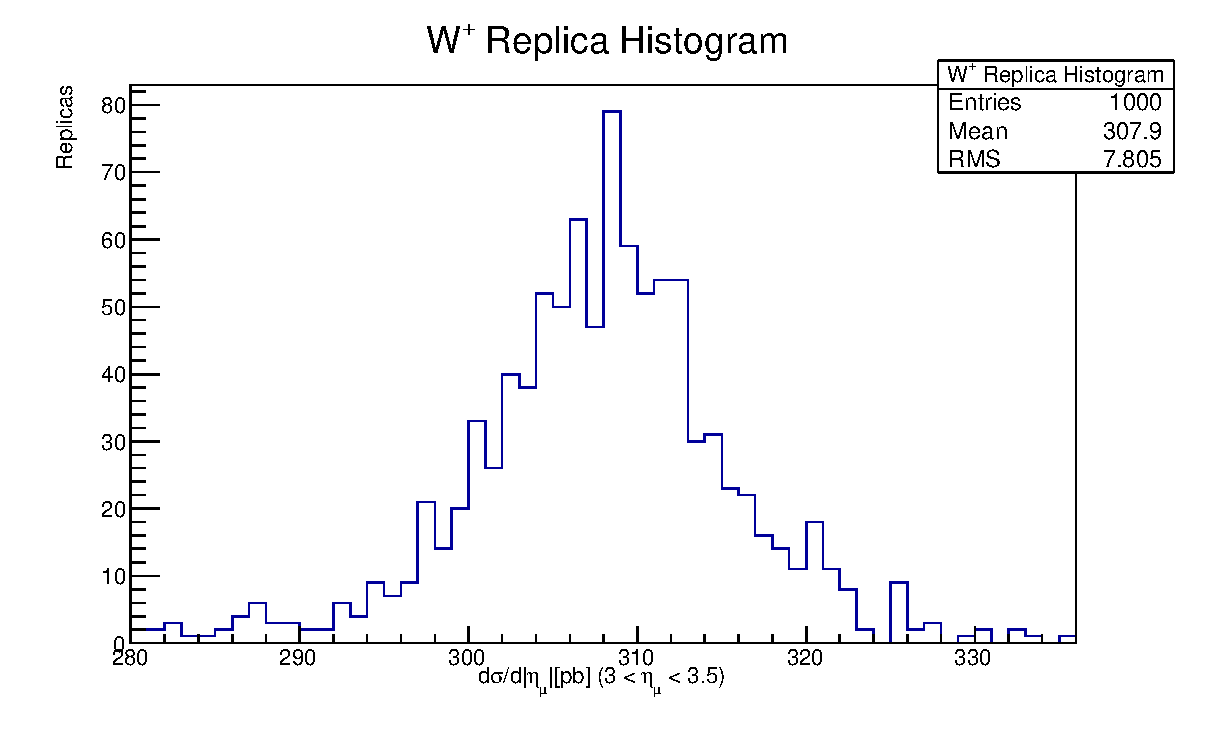
\includegraphics[width=\textwidth]{WpHist.eps}
\end{column}
\end{columns}

\vso
\center{Uncertainties in the PDFs faithfully represent the experimental data. \\No tolerance criterion is required.}

\end{frame}

%\begin{frame}
%\frametitle{The NNPDF Methodology }
%
%\begin{itemize}
%		\item<1-> Neural Network parametrization of PDFs \\
%		{ \color{blue} Redundant parametrization for an unbiased fit.}\vso
%		\item<1-> Monte Carlo uncertainty determination.\\
%		{ \color{blue}Faithful representation of the experimental uncertainties.}\vso
%		\item<1-> Genetic Algorithm for minimisation. \\
%		{ \color{blue}Efficient minimisation in a large parameter space.}\vso
%		\item<1-> Dynamical fit stopping by cross-validation. \\
%		{ \color{blue} Preventing overfitting.}
%		
%	\end{itemize}
%	
%	
%\end{frame}


\begin{frame}
\frametitle{Parton distributions for the LHC}
\vskip-10pt
\vskip-10pt
\vskip-10pt

\begin{itemize}
		\item<1-> Need to have a reliable determination of PDFs for LHC physics!
		\item<1-> For many EW processes PDF uncertainty dominates - good uncertainty analysis is crucial.
\end{itemize}
\vskip30pt
{ \usebeamerfont{title}  \color{lavendar} The LHC for parton distributions }
\vskip20pt

\begin{itemize}
		\item<1-> LHC can access PDFs in new kinematic regions $\to$ high $Q^2$ and small-$x$.
		\item<1-> LHC measurements starting to be able to discriminate between PDF sets.
\end{itemize}
	
\end{frame}

\begin{frame}
\frametitle{ NNPDF collider only fits }

\underline{Target}: An NNPDF Fit based only upon collider data
\begin{itemize}
\item<1-> Free of contamination from higher twist corrections.
\item<1-> Includes only proton data - no nuclear corrections required
\end{itemize}

 \begin{figure}[b!]
    \begin{center}
      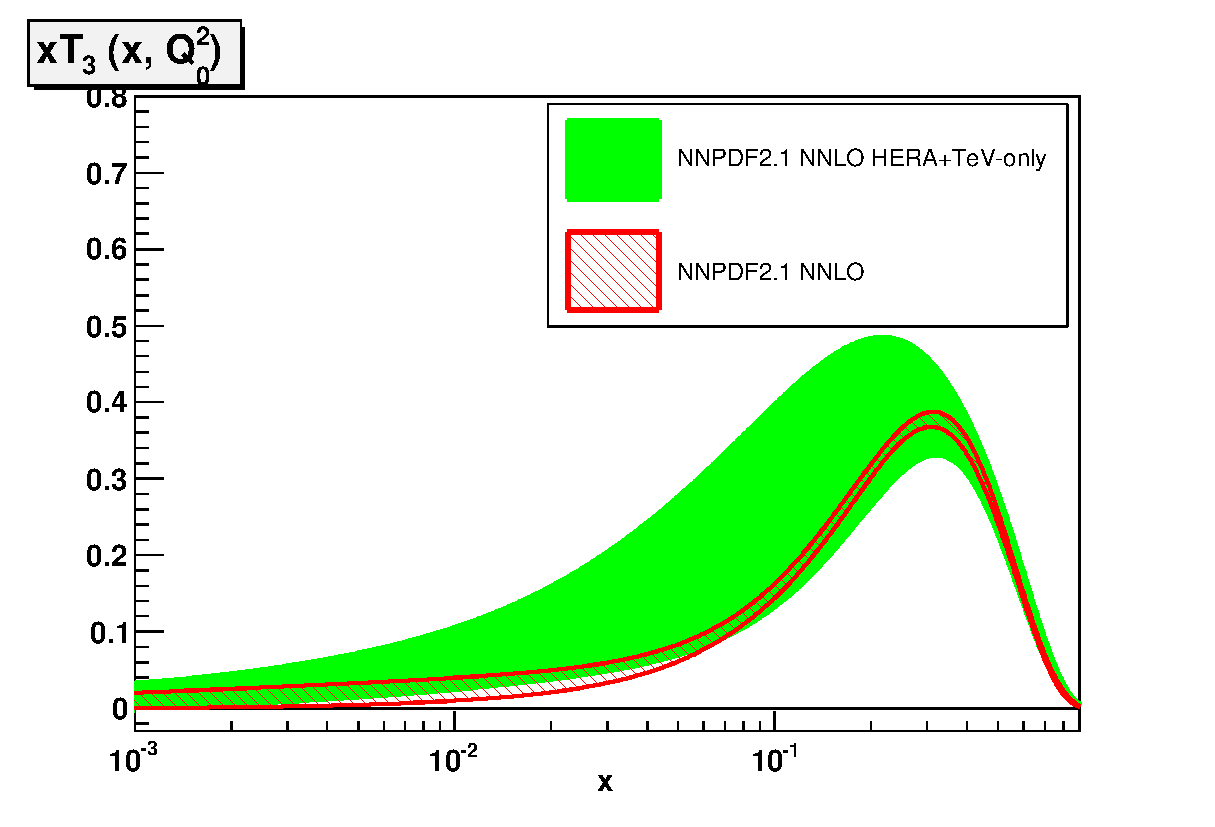
\includegraphics[width=0.50\textwidth]{xT3_Q_2_log-nnpdf21nnlo-collider.eps}
      \includegraphics[width=0.50\textwidth]{xSinglet_Q_2_log-nnpdf21nnlo-collider.eps}
    \end{center}
    \vskip-0.5cm
    \label{fig:pdf-jets}
\end{figure}
\begin{itemize}
\item<1->HERA + Tevatron data provide insufficient constraints in an NNPDF fit
\end{itemize}

\begin{itemize}
\item<1-> LHC data will be crucial to properly constrain future collider only NNPDFs
\end{itemize}
\end{frame}


\begin{frame}
\frametitle{ Strange content of the proton }
\begin{itemize}
\item<1-> Strange PDFs are relatively poorly constrained by existing data.
\begin{itemize}
\item<1-> Primary constraints from dimuon production in Neutrino DIS
\end{itemize}
\end{itemize}

\small {\be s^+(x) = s(x) + \bar{s}(x), \quad \quad\quad s^-(x) = s(x) - \bar{s}(x). \ee}
 \begin{figure}[b!]
    \begin{center}
      \includegraphics[width=0.50\textwidth]{pdf_xsplus_log_band_comparison_others.eps}
      \includegraphics[width=0.50\textwidth]{pdf_xsminus_band_comparison.eps}
    \end{center}
    \vskip-0.5cm
    \label{fig:pdf-jets}
\end{figure}


\begin{itemize}
\item<1-> Situation is much worse in collider only fits
\end{itemize}

\end{frame}



\begin{frame}
\frametitle{ LHC Data for PDFs - EW vector boson production  }


\begin{columns}

	\begin{column}{0.5\textwidth}
	
	\begin{itemize}
\item<1-> $pp \to W+X \to l\nu + X$ \\ $pp\to Z+X \to l^{+}l^{-} + X$
	\begin{itemize}
\item<1-> Potentially a vital constraint upon light flavour separation.
\end{itemize}
	\begin{itemize}
\item<1-> Strange contribution \textbf {much} more important that at Tevatron.
\end{itemize}
\end{itemize}
\vskip15pt

\begin{itemize}
\item<1-> $pp \to W+c+X $
	\begin{itemize}
\item<1-> Direct probe of strange distribution $(|V_{cs}|>|V_{cd}|)$
\end{itemize}
	\begin{itemize}
\item<1-> May provide important constraint upon strange valence distribution.
\end{itemize}
\end{itemize}
	
\end{column}

	\begin{column}{0.5\textwidth}
 \begin{figure}[b!]
    \begin{center}
      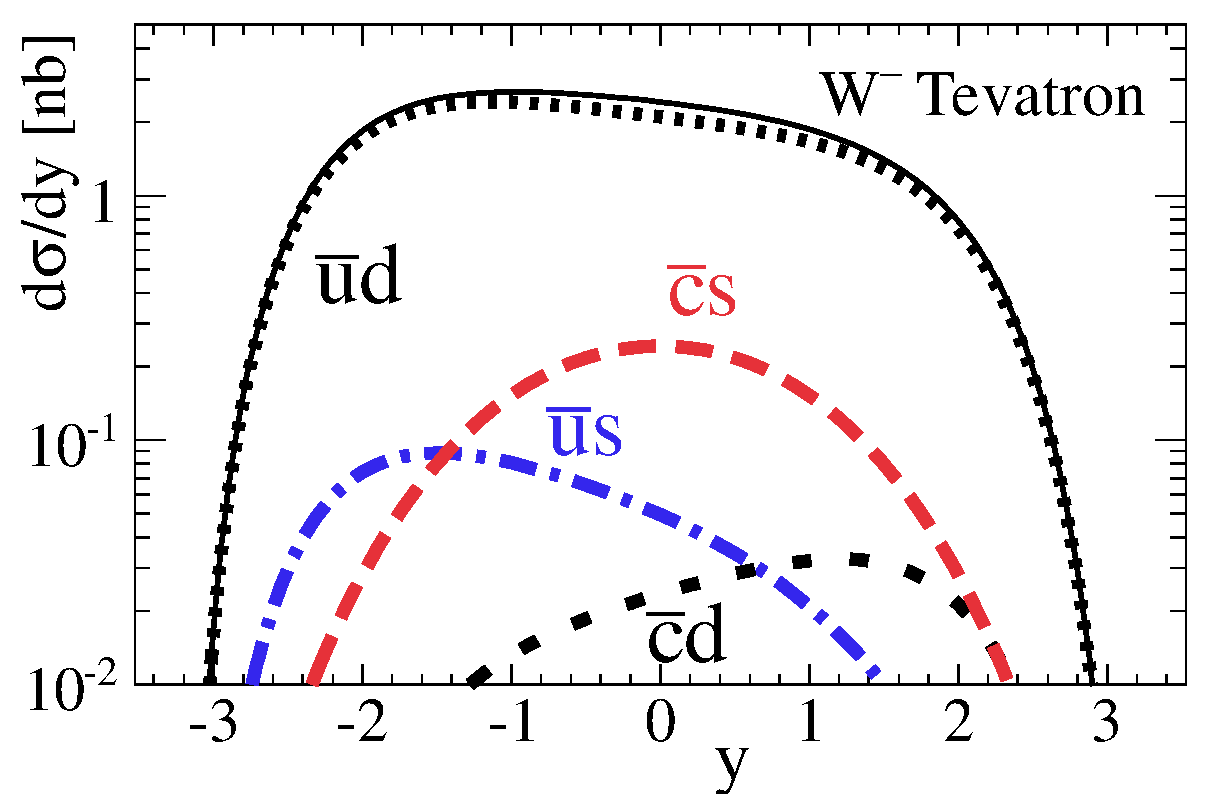
\includegraphics[width=0.5\textwidth]{WmTEV.eps}
       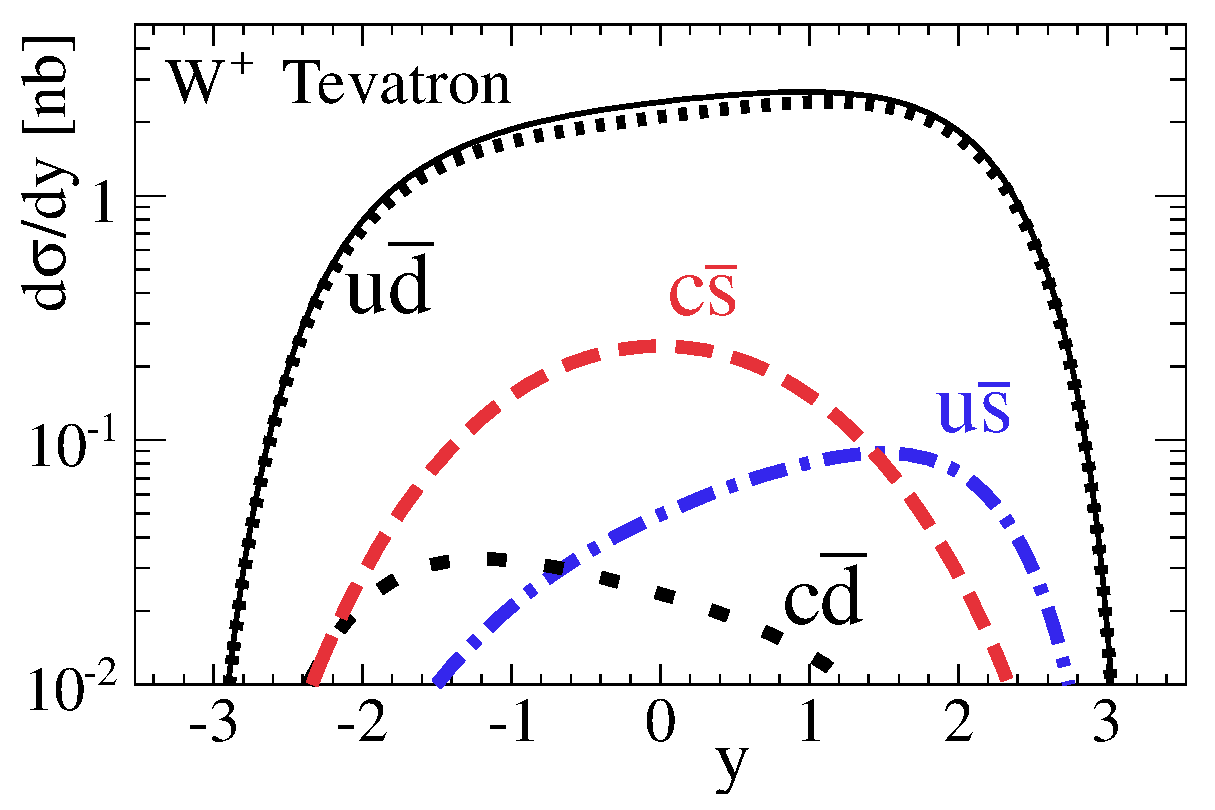
\includegraphics[width=0.5\textwidth]{WpTEV.eps}\\
      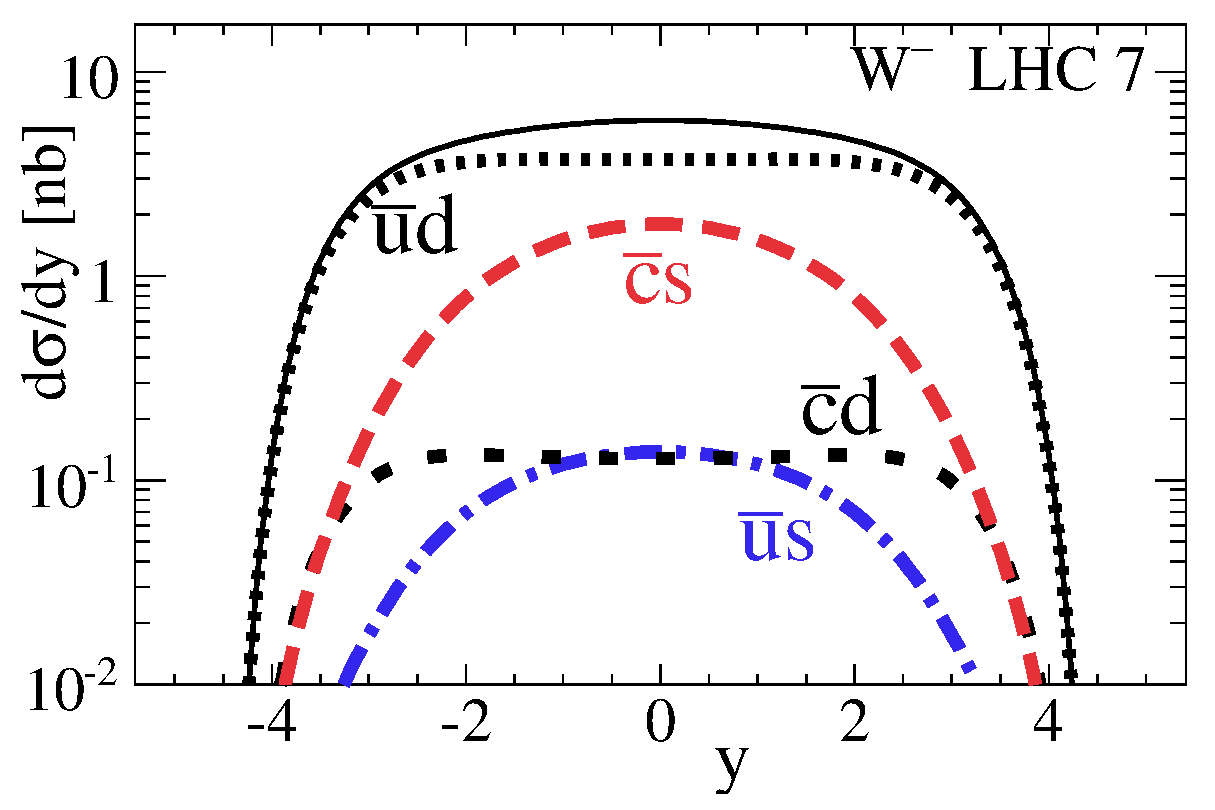
\includegraphics[width=0.5\textwidth]{WmLHC7.eps}
       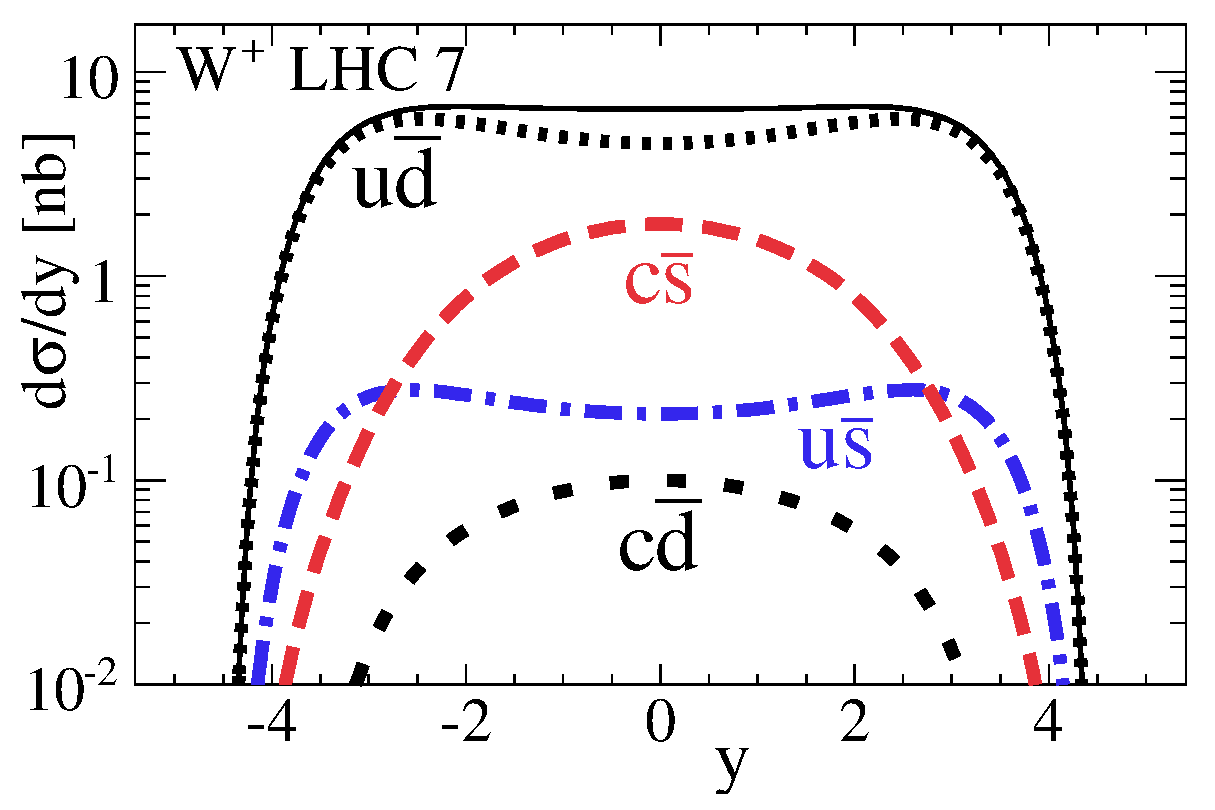
\includegraphics[width=0.5\textwidth]{WpLHC7.eps}\\
      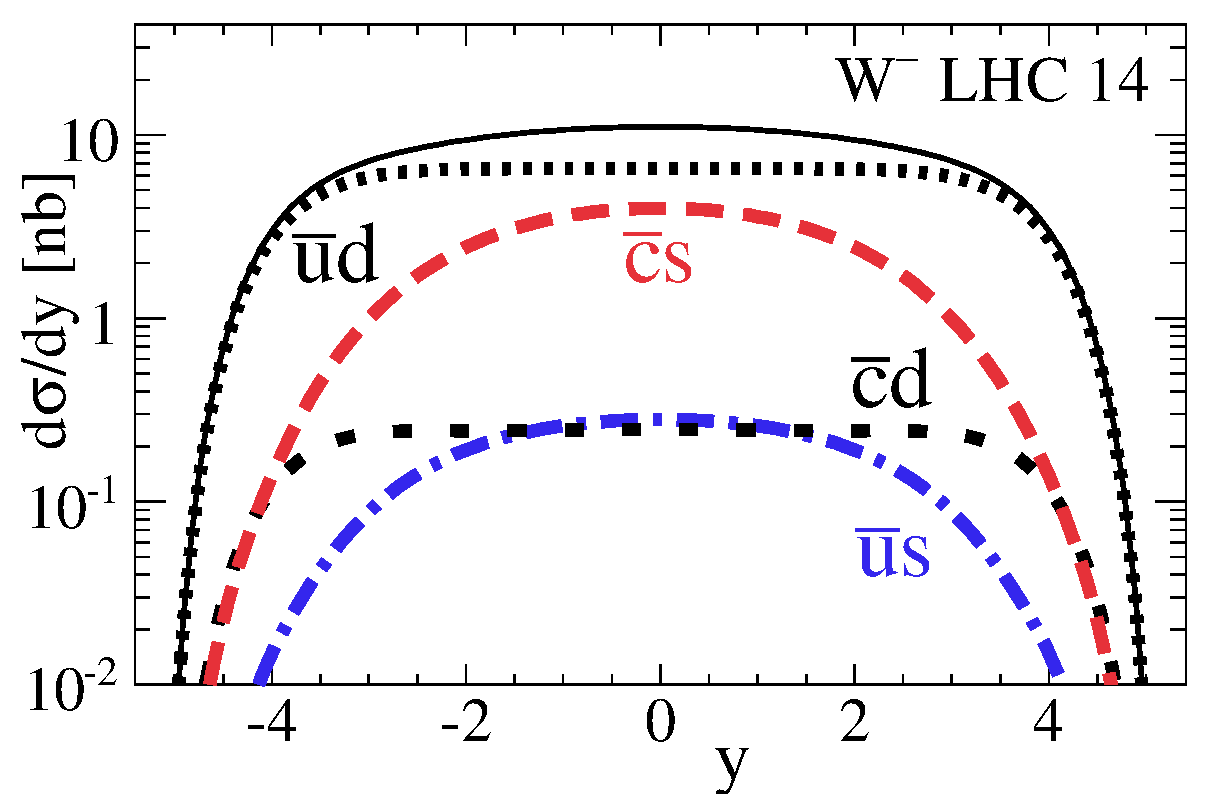
\includegraphics[width=0.5\textwidth]{WmLHC14.eps}
       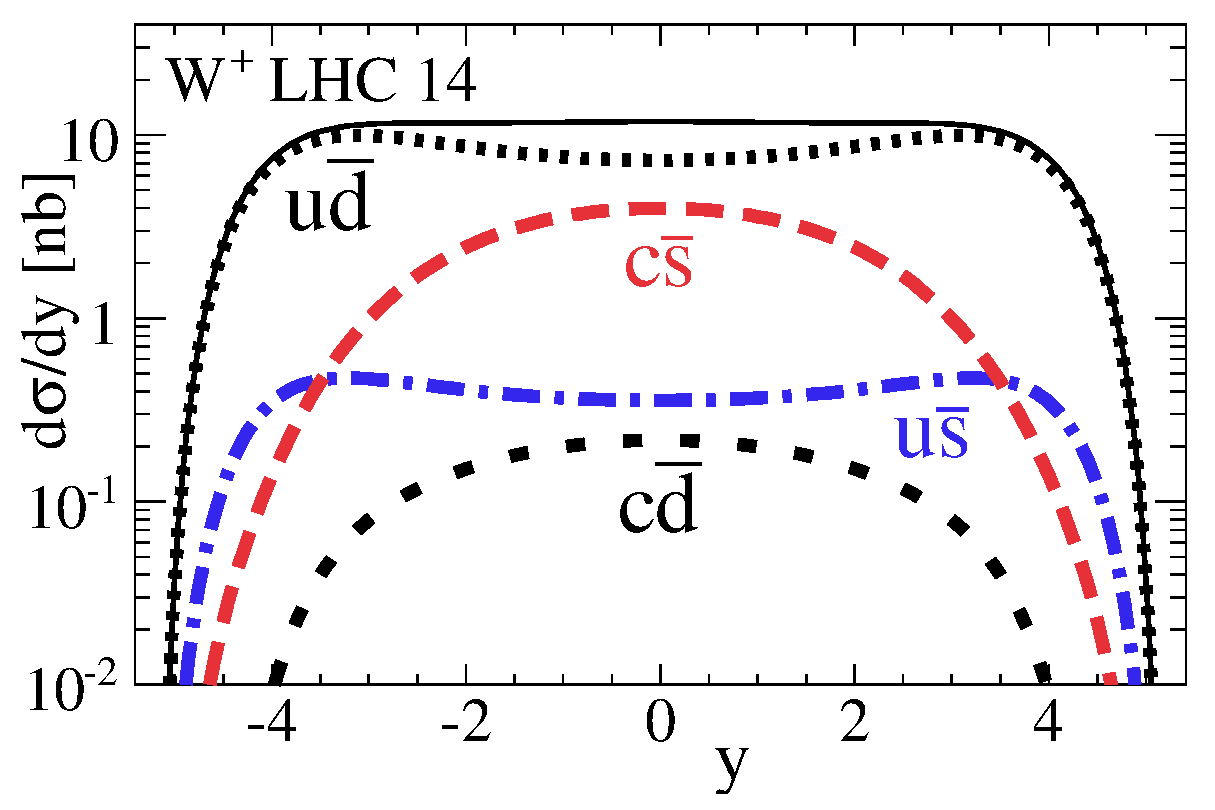
\includegraphics[width=0.5\textwidth]{WpLHC14.eps}\\
    \end{center}
    \vskip-0.5cm
    \label{fig:pdf-jets}
\end{figure}

{ \footnotesize \hfill A. Kusina \emph{et al} [arXiv:1203.1290] }

\end{column}

\end{columns}

\end{frame}


\begin{frame}
\frametitle{LHC Data for PDFs - Inclusive Jets }
\begin{itemize}
\item<1-> Precision inclusive jet data important for constraining the gluon distribution. 
\end{itemize}
 \begin{figure}[b!]
    \begin{center}
      \includegraphics[width=0.50\textwidth]{pdf_xg_band_comparison.eps}
       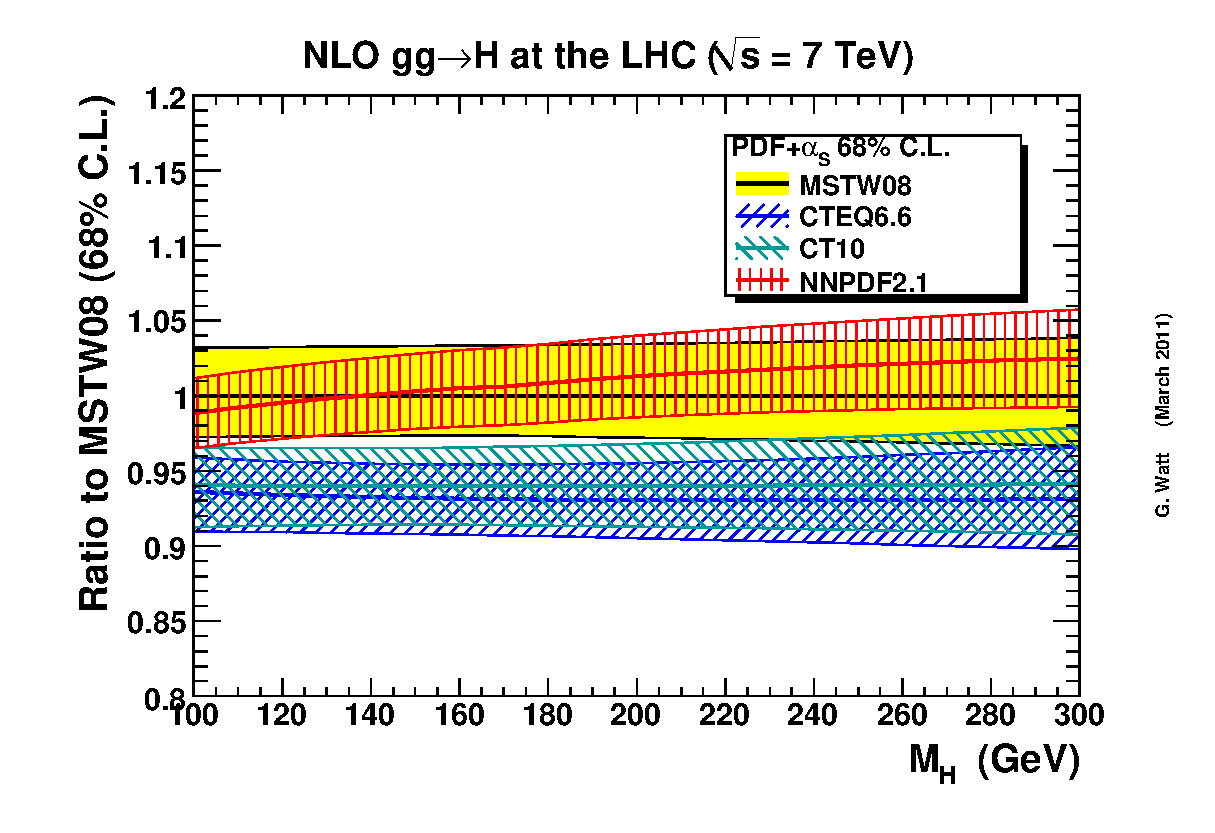
\includegraphics[width=0.50\textwidth]{ratioggHLHC7TeV68cl_noasth.eps}
    \end{center}
    \vskip-0.5cm
    \label{fig:pdf-jets}
\end{figure}
\begin{itemize}
\item<1-> Much of the current large-$x$ constraints upon the gluon distribution are due to Tevatron jet data. 
\item<1-> Precise LHC measurements could provide valuable constraints.
\end{itemize}
\end{frame}





\begin{frame}
\frametitle{Including new experimental data}
How can we add new data to an existing parton set?

\begin{itemize}
		\item<1-> Perform a new fit.\\
		{\small (Difficult if a fast implementation of the theoretical prediction is not available).}
		\item<1-> Reweight existing Monte Carlo parton set. {\small \color{blue} Giele, Keller [hep-ph/9803393] }\\
\end{itemize}
If the new data is statistically independent of the data in the prior set:
\be
\mathcal{P}_{\rm new}(f)
= \mathcal{N}_{\chi}\mathcal{P}(\chi^2|f)\;\mathcal{P}_{\rm old}(f),
\ee
		\be \langle\mathcal{O}\rangle_{\mathrm {new}}=\int \mathcal{O}[f] \, \mathcal{P}_{ \mathrm {new}}(f)\,Df=\smallfrac{1}{N}\,\sum_{k=1}^{N}w_k\mathcal{O}[f_k].\,  \ee
Weights determined by statistical inference
\be w_k =\mathcal{N}_\chi\mathcal{P}(\chi^2|f_k) = 
\frac{(\chi^{2}_k)^{(n-1)/2} 
e^{-\frac{1}{2}\chi^{2}_k}}
{\smallfrac{1}{N}\sum_{k=1}^{N}(\chi^{2}_k)^{(n-1)/2}
e^{-\frac{1}{2}\chi^{2}_k}}\, .\ee
\center{ \small  R.~D.~Ball {\it et al.} Nucl.\ Phys.\ B {\bf 849} 112  [arXiv:1012.0836]. }

\end{frame}

\begin{frame}
\frametitle{Ensemble Efficiency}

   \begin{itemize}
		\item<1-> Prior set: maximally efficient representation of probability distribution.
		\item<1-> Reweighted set: loss of efficiency due to very small weights.
		\item<1-> Many replicas no longer contribute to the ensemble.
\end{itemize}

\center{Loss of information quantified by the Shannon entropy:}
  \be N_{\textrm{ eff}} \equiv \exp \left(\frac{1}{N_{\mathrm{rep}}}\sum_{k=1}^{N_{\mathrm{rep}}}w_k\ln(N_{\mathrm{rep}}/w_k)\right)\ee
\begin{columns}
  \begin{column}{0.45\textwidth}
 \begin{figure}[b!]
    \begin{center}
      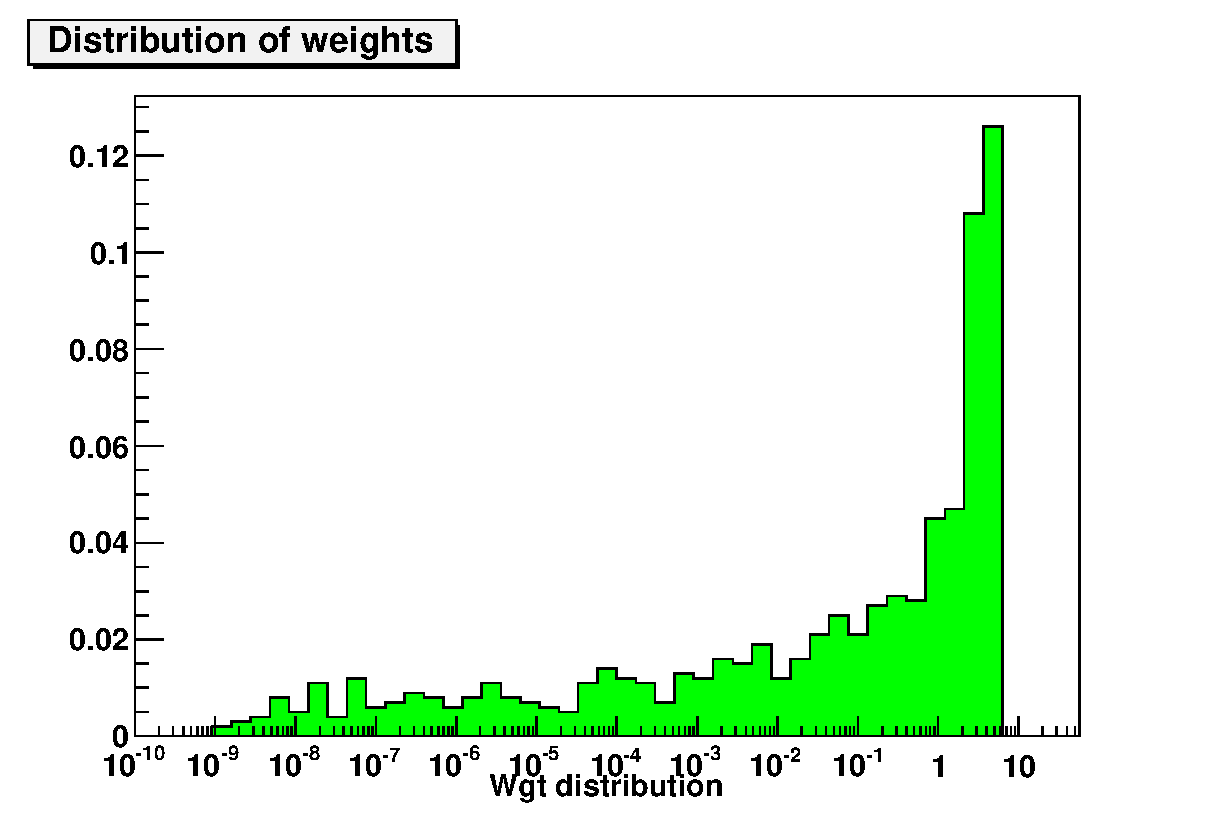
\includegraphics[width=0.85\textwidth]{wgt-dist-jets-t0.eps}
    \end{center}
\end{figure}

  \end{column}

  \begin{column}{0.55\textwidth}
  A very low $N_{\textrm{ eff}}$ means data is either:
 \begin{itemize}
		\item<1-> Very constraining
		\item<1-> Inconsistent with prior
\end{itemize}
\vskip10pt
     \end{column}
\end{columns}
\end{frame}

\begin{frame}
\frametitle{Error rescaling parameter}
Useful tool for analysing experimental uncertainties. 
Differentiates between inconsistent and constraining data when $N_{\mathrm{eff}}$ is small.
\begin{itemize}
		\item<1-> Rescale uncertainties by a factor $\alpha$.
		\item<1-> Compute a new weight $w_k(\alpha)$ with these uncertainties.
		\item<1-> Average over all replicas $\to$ probability of rescaling uncertainties by $\alpha$.
\end{itemize}


\begin{columns}
  \begin{column}{0.5\textwidth}
  \begin{block}{}
\be \chi^2_{k,\alpha} = \chi^2_k/\alpha^2, \ee
\be w_k(\alpha) = (\chi^2_{k,\alpha})^{(n-1)/2}\mathrm{e}^{-\chi^2_{k,\alpha}/2,}\ee
\be \mathcal{P}(\alpha | \chi^2)\propto \smallfrac{1}{\alpha}\sum_{k=1}^N w_k(\alpha).\ee
\end{block}
  \end{column}
  
    \begin{column}{0.5\textwidth}
 \begin{figure}[b!]
    \begin{center}
      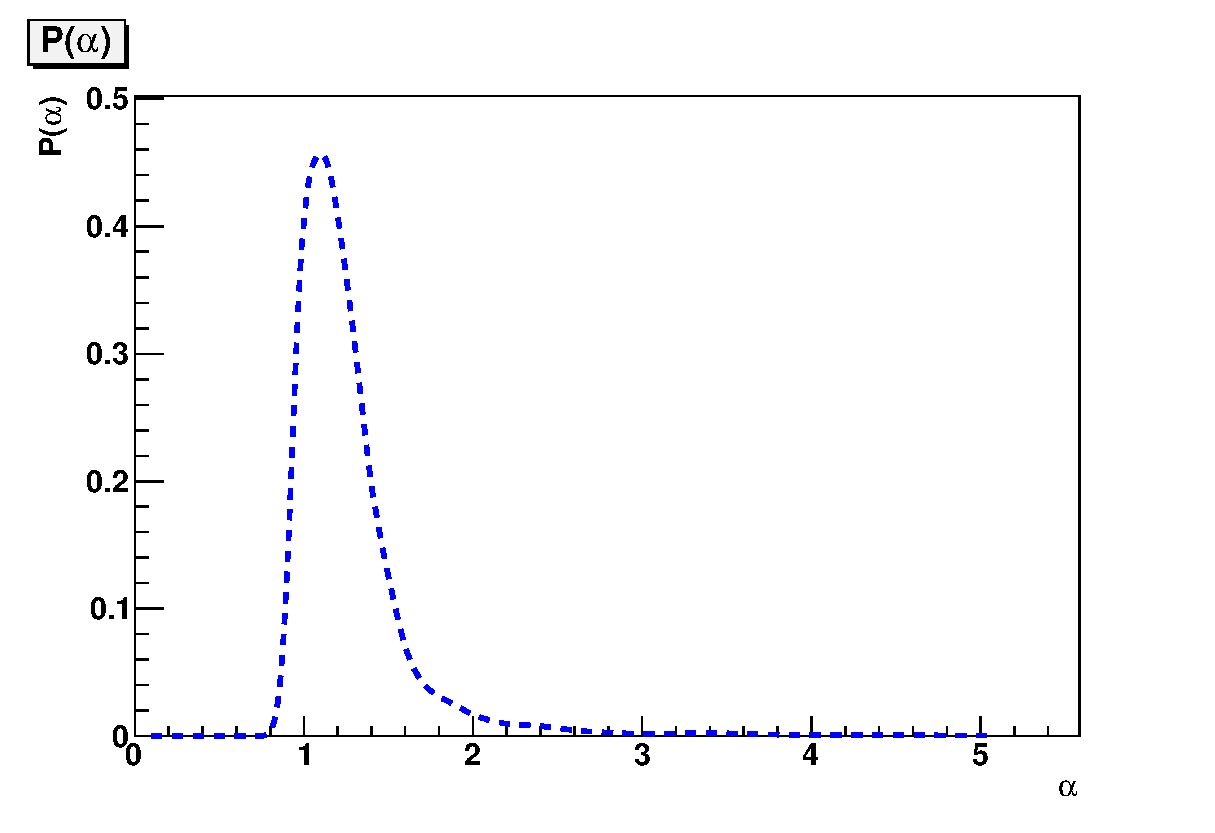
\includegraphics[width=1\textwidth]{palpha-jets-t0.eps}
    \end{center}
\end{figure}

  \end{column}  
  \end{columns}

\begin{figure}[b!]
    \begin{center}
    \end{center}
    \vskip-0.5cm

\end{figure}

\end{frame}


\begin{frame}
\frametitle{Reweighting Application: W+c Pseudodata}

\begin{itemize}
		\item<1-> \small Generate MC pseudo data for W+c events with CMS kinematics 
		\item<1-> \small Reweight NNPDF2.1 fit with artificial data to investigate possible impact of high statistics measurements.
\end{itemize}
\includegraphics[width=\textwidth]{wCrw.png}
\begin{itemize}
		\item<1-> \small Suggests substantial constrain possible with 5fb$^{-1}$
		\item<1-> \small Brings collider only strangeness to $\sim$ same accuracy as global fit.
		\item<1-> \small After $5$fb$^{-1}$ uncertainties are systematics dominated $\to$ W+jets.

\end{itemize}
\vskip20pt
\hfill (J.Rojo)
\end{frame}



\begin{frame}
\frametitle{Reweighting Application: NNPDF2.2 Parton Set .}
New data added by reweighting NNPDF2.1 Fit: $W$ leptonic charge asymmetry.
\begin{centering}
\center{\small  R.~D.~Ball {\it et al}, Nucl.\ Phys.\ B {\bf 855} 608 {\color{blue} [arXiv:1108.1758] }.}\\
\end{centering}\vskip5pt
Defined in terms of $W^{\pm}\to l^\pm\nu_l $ differential cross-sections $d\sigma_{l^\pm}/d\eta_l$
\be 
  A^l_W=\frac{d\sigma_{l^{+}}/d\eta_{l}-d\sigma_{l^{-}}/d\eta_{l}}
  {d\sigma_{l^{+}}/d\eta_{l}+d\sigma_{l^{-}}/d\eta_{l}}, 
\ee

\begin{itemize}
		\item<1-> ATLAS $\mu$ charge asymmetry. \hspace*{\fill {  \color{blue} [arXiv:1103.2929]}}
		\item<1-> CMS $e+\mu$ charge asymmetry. \hspace*{\fill { \color{blue}  [arXiv:1103.3470] }}
		\item<1-> D0 $e+\mu$ charge asymmetry. \hspace*{\fill { \color{blue} [arXiv:0709.4254]}}
\end{itemize}

\begin{figure}[h!]
  \centering
  \epsfig{width=0.44\textwidth,figure=xu-nnpdf22.eps}
  \epsfig{width=0.44\textwidth,figure=xd-nnpdf22.eps}
\end{figure}

\end{frame}
 \begin{frame}
\frametitle{Including new experimental data - fitting}
How can we efficiently include LHC data into a full fit?

\underline{Tools}: APPLgrid/FastNLO projects 

\begin{itemize}
\item<1-> Precompute and store MC weights on an interpolation grid in $x$ and $Q^2$:
\end{itemize}
 \be \sigma= \sum_p \sum_{l}^{N_{\mathrm{sub}}} \int_0^1 dx_1dx_2\; \hat{\sigma}^{(p)(l)} \left( x_1,x_2,Q^2 \right)  F^{(l)}\left(x_1, x_2,  Q^2 \right) \to \ee

\begin{equation}
\label{eq:applconv}
\sigma = \sum_p \sum_{l}^{N_{\mathrm{sub}}} \sum_{\alpha,\beta}^{N_x} \sum_{\tau}^{N_{Q}}
W_{\alpha\beta\tau}^{(p)(l)} \,
F^{(l)}\left(x_{\alpha}, x_{\beta},  Q^2_{\tau}\right)
\end{equation}
PDF Evolution in the FastKernel method is a similar procedure,
\underline{Idea}: Combine weight grids with evolution grids 
\be f_i(x_{\alpha},Q^2_\tau) =  \sum_\beta^{N_{x}} \sum_{j}^{N_{\mathrm{pdf}}} A^{\tau}_{\alpha\beta ij}N^0_j(x_{\beta} ) \quad \to \quad
 \sigma= \sum_{\alpha,\beta}^{N_x}\sum_{i,j}^{N_{\mathrm{pdf}}} \sigma_{\alpha\beta i j}N_i^0(x_\alpha)N_j^0(x_\beta)
\ee 
 \begin{itemize}
\item<1-> Precomputing all $Q^2$ dependence leads to extremely efficient calculations.
\end{itemize}\end{frame}

\begin{frame}
\frametitle{NNPDF2.3 - LHC Data}
\begin{itemize}
\item<1->{ \small The NNPDF2.3 dataset contains all relevant LHC data with covariance matrices }
 \begin{itemize}
 \item<1->  $36$ pb$^{-1}$ ATLAS Inclusive jet measurements \hfill  {\color{blue}[arxiv:1112.5141]}
  \item<1->  $35$ pb$^{-1}$  ATLAS W lepton and Z differential distributions \hfill{\color{blue}[arxiv:1109.5141]}
   \item<1->  $37$ pb$^{-1}$ LHCb W lepton differential distribution \hfill {\color{blue}[arxiv:1204.1620]}
  \item<1-> $840$ pb$^{-1}$ CMS  W electron asymmetry \hfill {\color{blue}[arxiv:1206.2598]}

\end{itemize}
\end{itemize}

\begin{columns}
  \begin{column}{0.5\textwidth}
   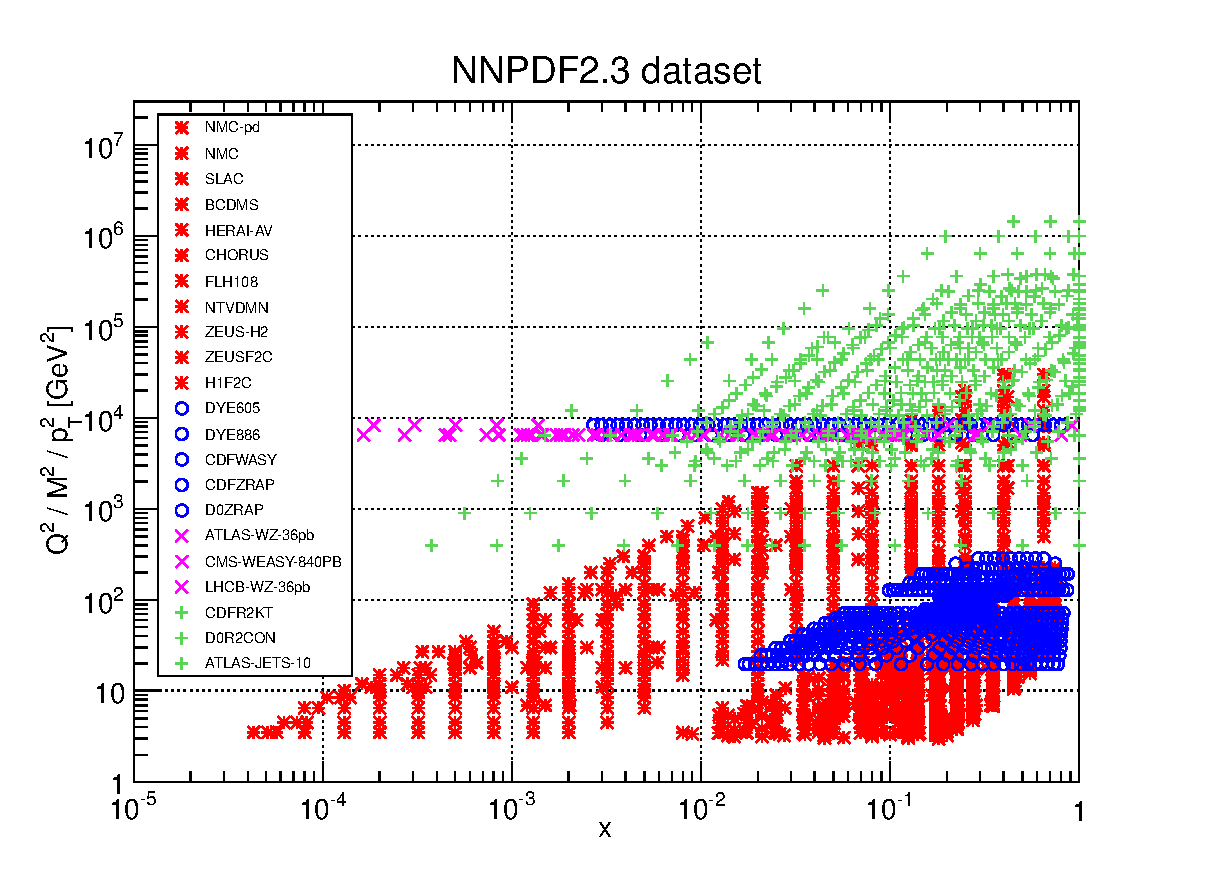
\includegraphics[width=1.0\textwidth]{kin23}
  \end{column}

  \begin{column}{0.5\textwidth}
    \small
\underline{Methodological Improvements}\\
\vskip10pt
Improved dynamical stopping.\\
Expanded genetic algorithm minimisation.\\
Improved training/validation partitioning. \\
Correction to NuTeV dimuon cross section.

\begin{table}
\scriptsize
\begin{tabular}{|c|c|c||c|c|}
\hline 
& \multicolumn{2}{c||}{\bf NNPDF2.1} & \multicolumn{2}{|c|}{\bf NNPDF2.3}  \\
\hline 
\hline 
  & NLO & NNLO  & NLO  & NNLO  \\
\hline 
Fit Quality  & 1.15 & 1.16  & 1.10 & 1.14     \\
\hline
\end{tabular}
\end{table}

  \end{column}
\end{columns}



\begin{itemize}
\item<2->Also in the NNPDF2.3 family
\begin{itemize}
 \item<1-> NNPDF2.3 noLHC:  same dataset as NNPDF2.1, with improved methodology.
  \item<1->  NNPDF2.3 Collider only: dataset restricted to HERA, Tevatron and LHC data.
\end{itemize}
\end{itemize}
\end{frame}


\begin{frame}
\frametitle{NNPDF2.3 Dataset}
   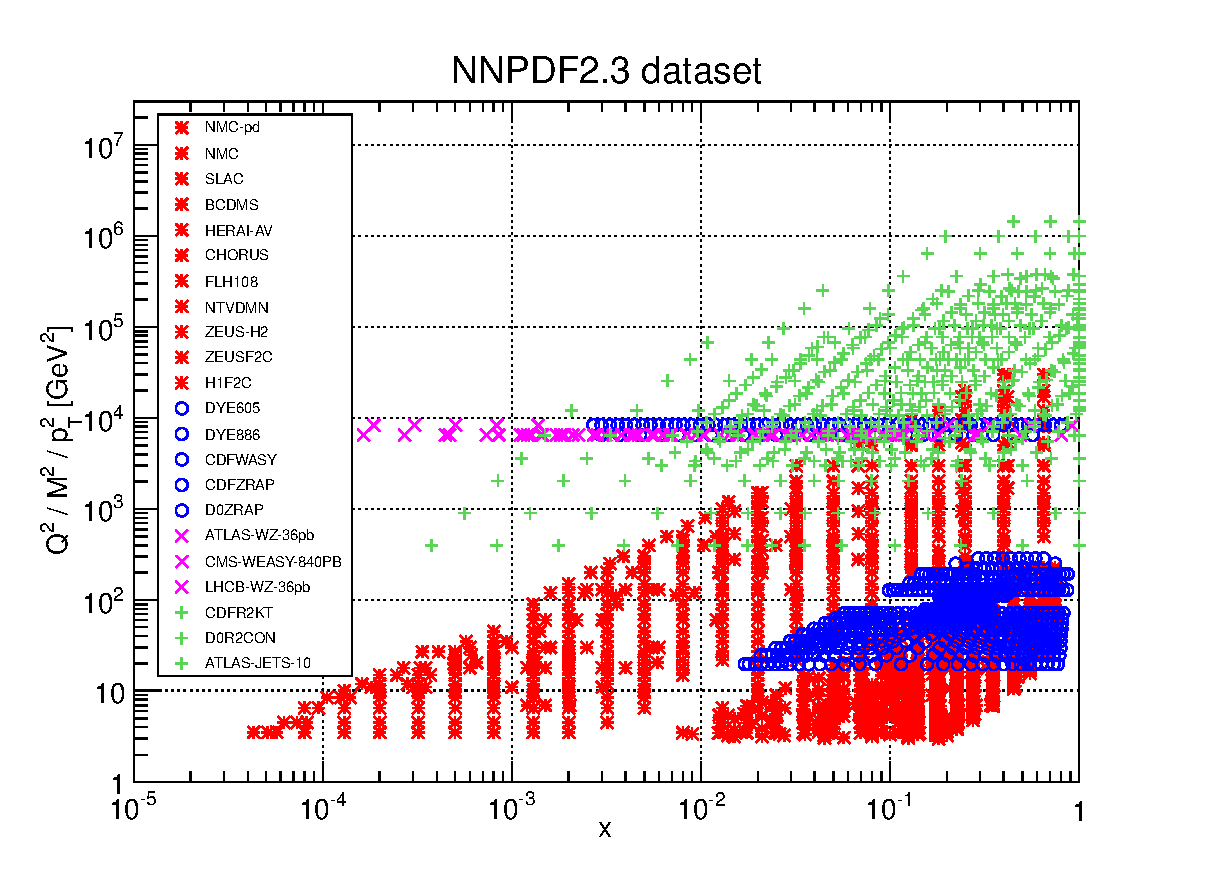
\includegraphics[width=1.0\textwidth]{kin23}
\end{frame}



\begin{frame}
\frametitle{Impact of LHC EW vector boson data}
 \begin{figure}[b!]
    \begin{center}
      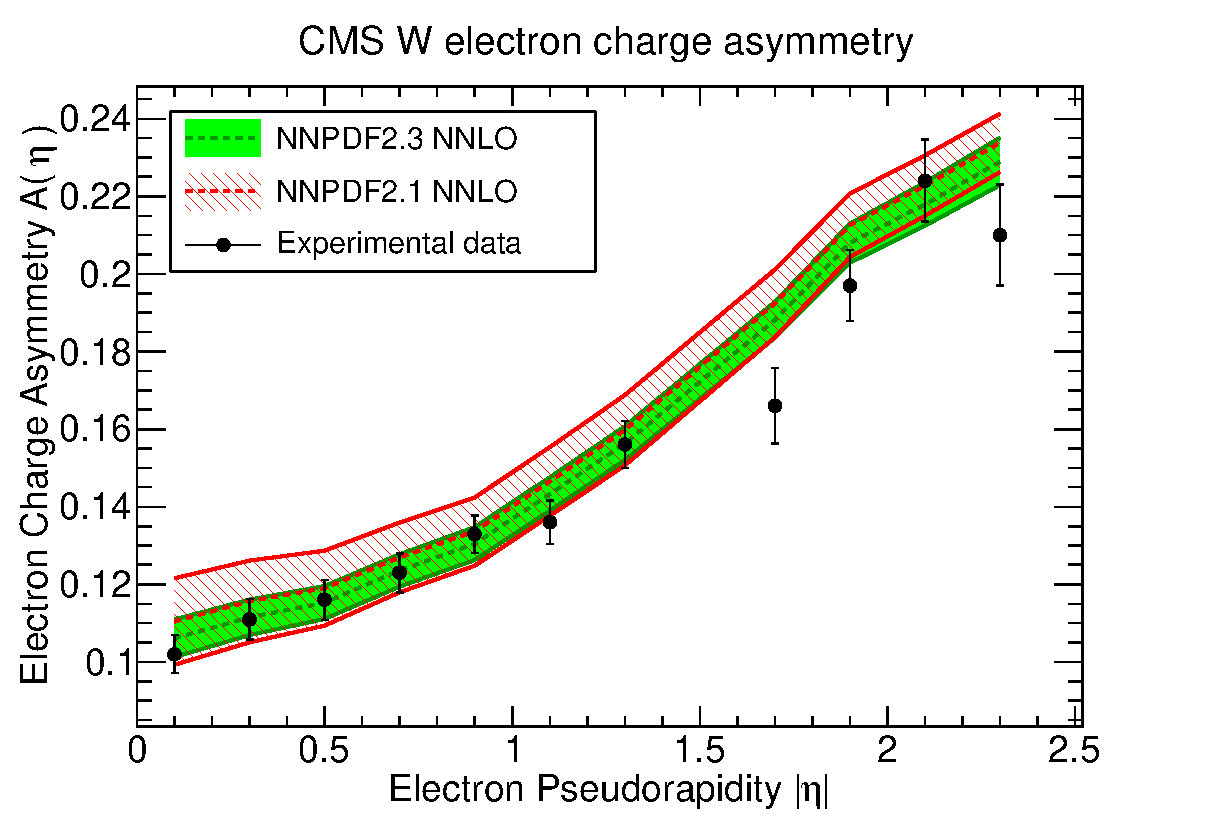
\includegraphics[width=0.50\textwidth]{CMSWEASY840PB_0.eps}
      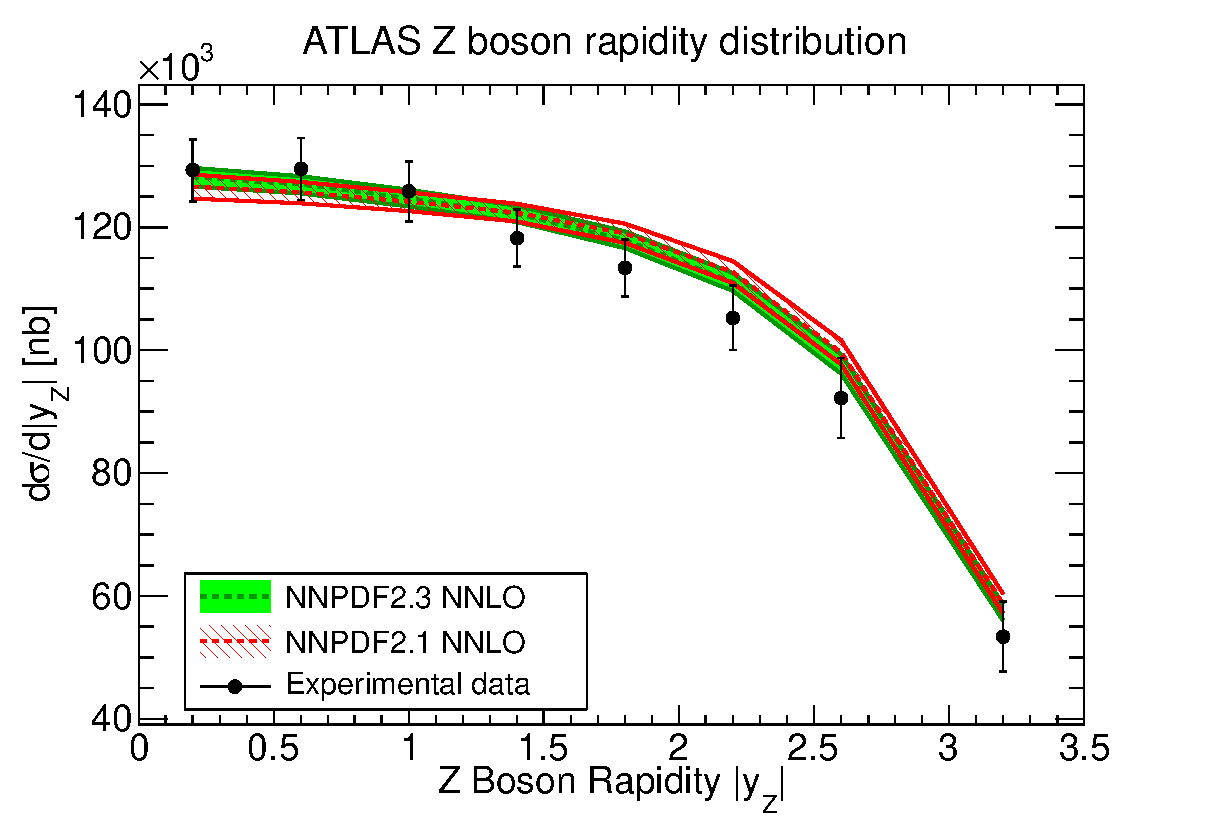
\includegraphics[width=0.50\textwidth]{ATLASWZRAP36PB_2.eps}
    \end{center}
    \vskip-0.5cm
    \label{fig:pdf-jets}
\end{figure}

\begin{table}
\small
\begin{tabular}{|c||c|c||c|c|}
\hline 
& \multicolumn{2}{c||}{\bf NNPDF2.1} & \multicolumn{2}{|c|}{\bf NNPDF2.3}  \\
\hline 
\hline 
Experiment  & NLO & NNLO  & NLO  & NNLO  \\
\hline
ATLAS W/Z Distributions & {\it 1.57} & {\it 2.21}  & 1.26  &  1.43   \\
CMS $W_e$ Asymmetry  & {\it 2.02} & {\it 1.27}  & 0.82 & 0.81   \\
LHCb W Distributions & {\it 0.89} &  {\it 1.13} & 0.67  & 0.83   \\
\hline
\end{tabular}
\end{table}


\end{frame}

\begin{frame}
\frametitle{Impact of ATLAS inclusive jet data}
 \begin{figure}[b!]
    \begin{center}
      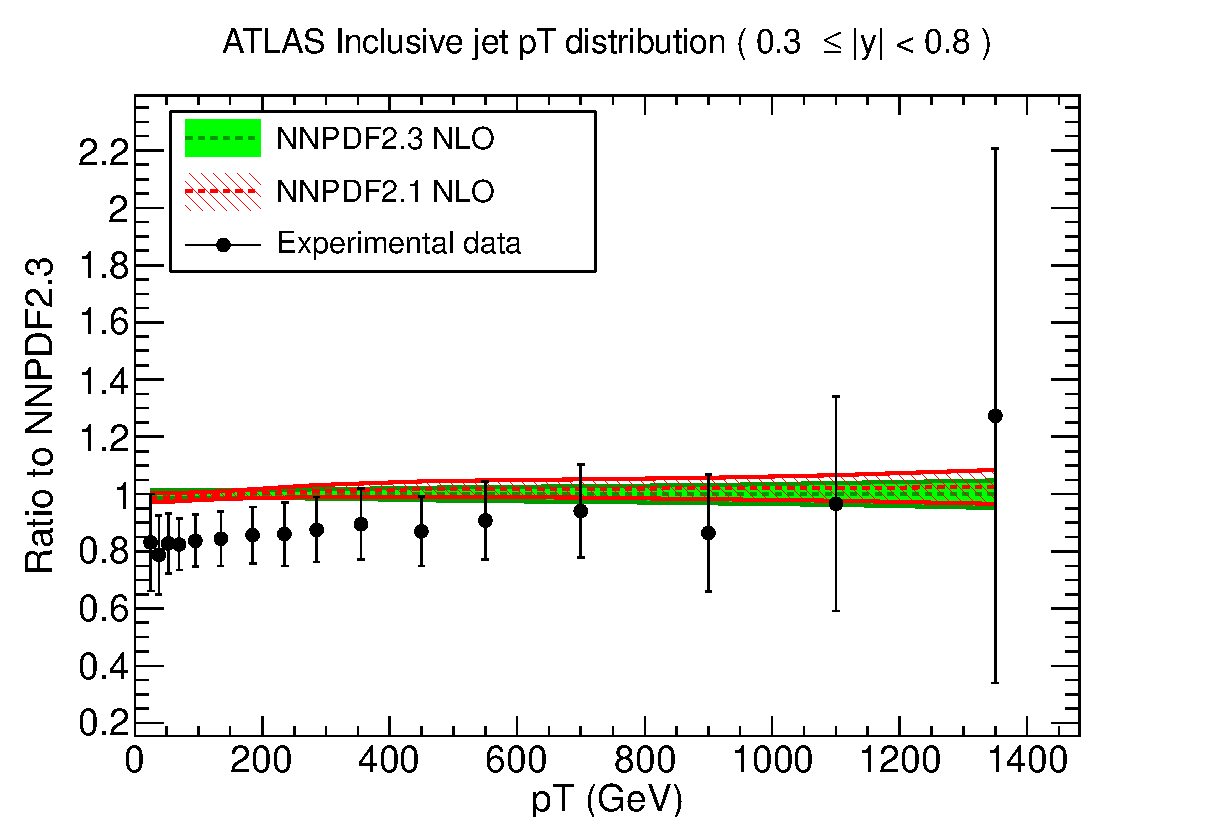
\includegraphics[width=0.50\textwidth]{ATLASR04JETS36PB_1}
      \includegraphics[width=0.50\textwidth]{ATLASR04JETS36PB_2}
    \end{center}
    \vskip-0.5cm
    \label{fig:pdf-jets}
\end{figure}
\begin{table}
\small
\begin{tabular}{|c||c|c||c|c|}
\hline 
& \multicolumn{2}{c||}{\bf NNPDF2.1} & \multicolumn{2}{|c|}{\bf NNPDF2.3}  \\
\hline 
\hline 
Experiment  & NLO & NNLO  & NLO  & NNLO  \\ 
\hline
ATLAS Inclusive Jets  & {\it 1.06} & {\it 0.95}  & 1.00  &  0.94   \\
\hline
\end{tabular}
\end{table}


\end{frame}

\begin{frame}
\frametitle{NNPDF2.3 vs NNPDF2.1}
 \begin{figure}[b!]
    \begin{center}
      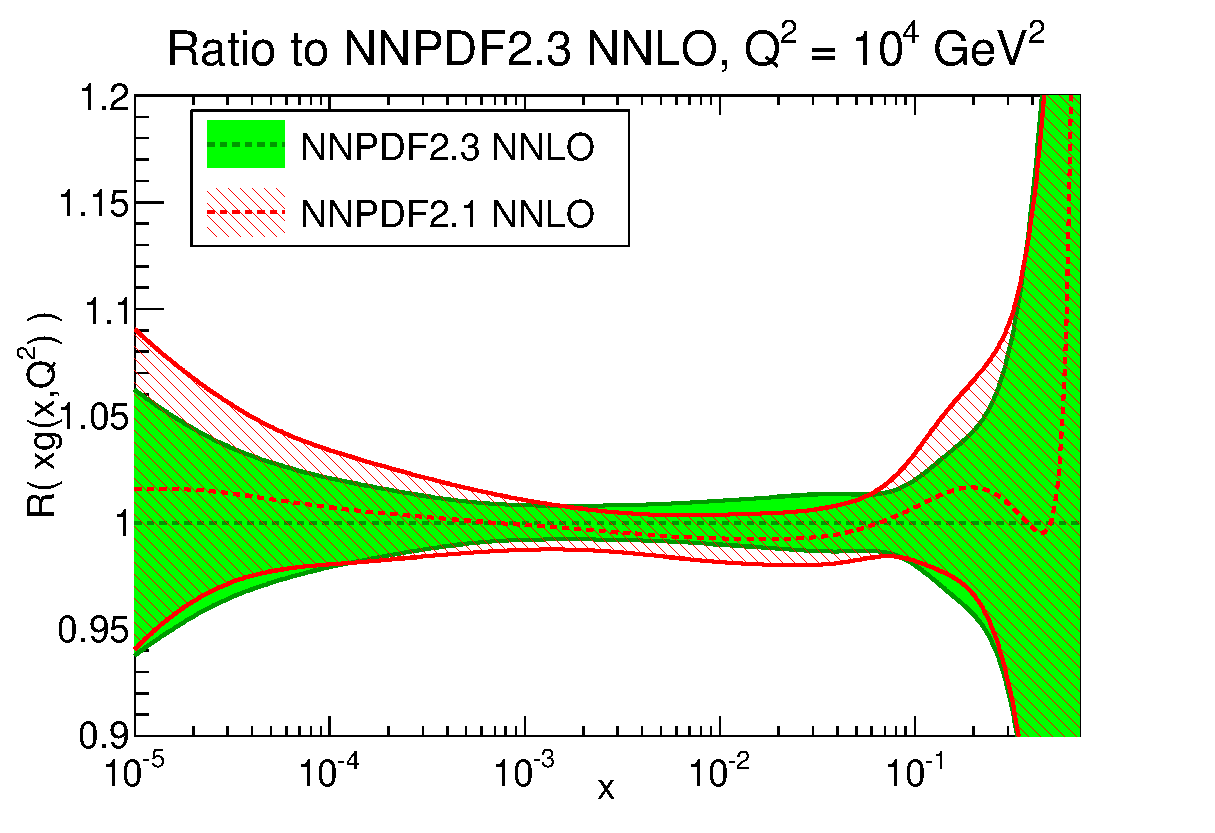
\includegraphics[width=0.50\textwidth]{xg_Q_10000_log-rat-21-vs-23-nnlo}
      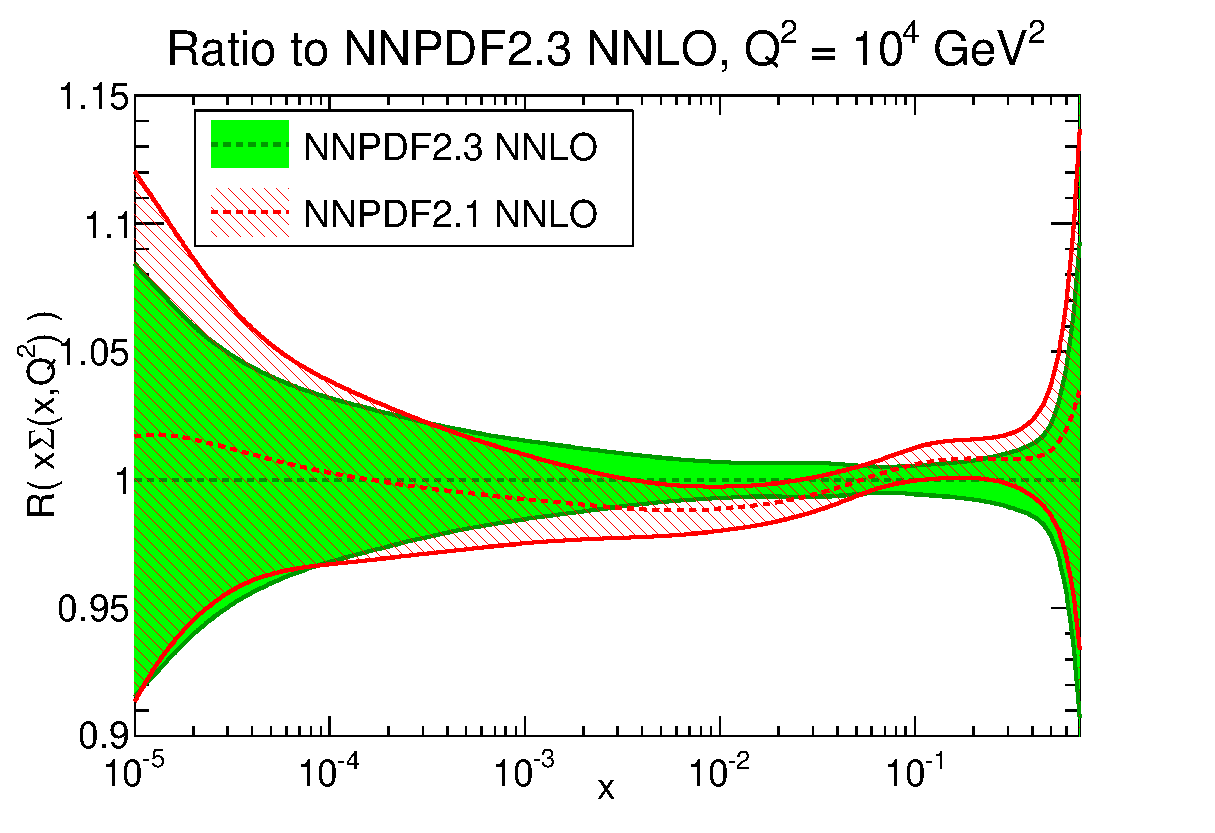
\includegraphics[width=0.50\textwidth]{xSinglet_Q_10000_log-rat-21-vs-23-nnlo}
    \end{center}
    \vskip-0.5cm
    \label{fig:pdf-jets}
\end{figure}

 \begin{figure}[b!]
    \begin{center}
      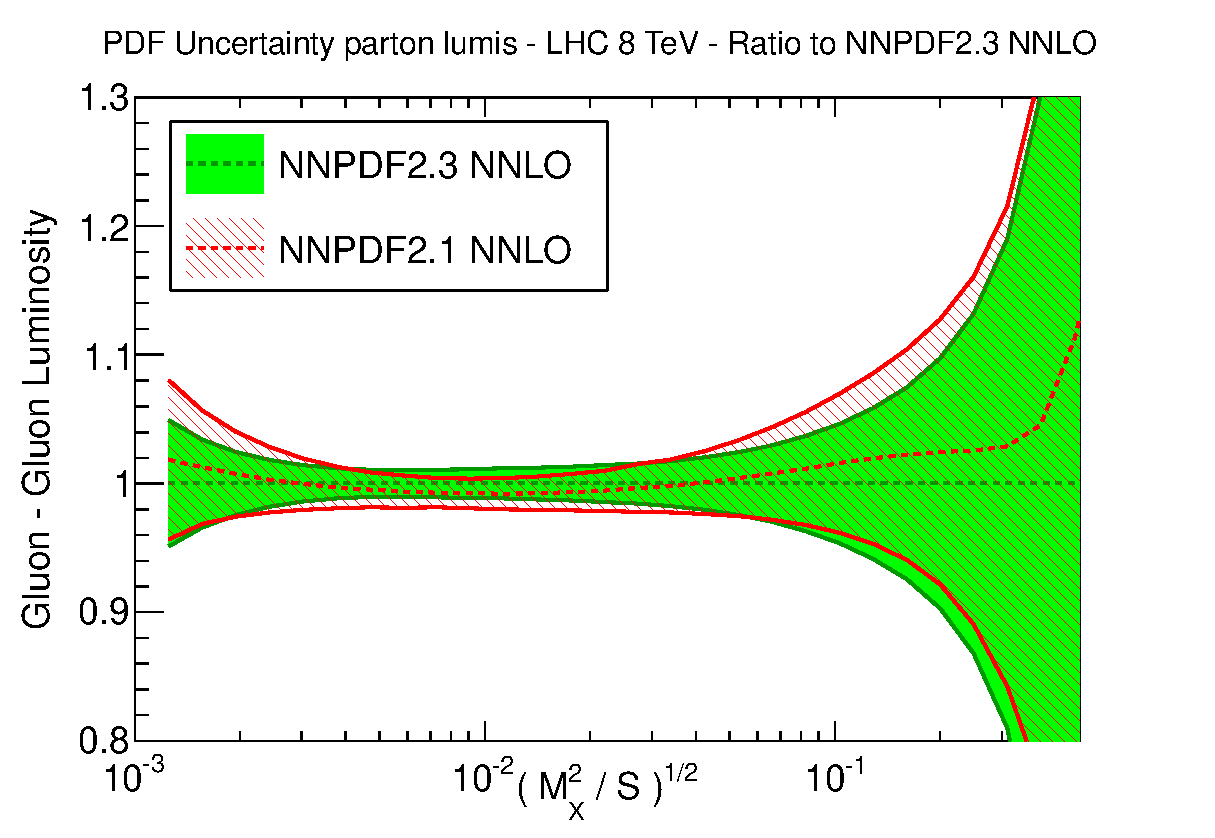
\includegraphics[width=0.50\textwidth]{gg_S_6_4e+07-rat-8tev}
      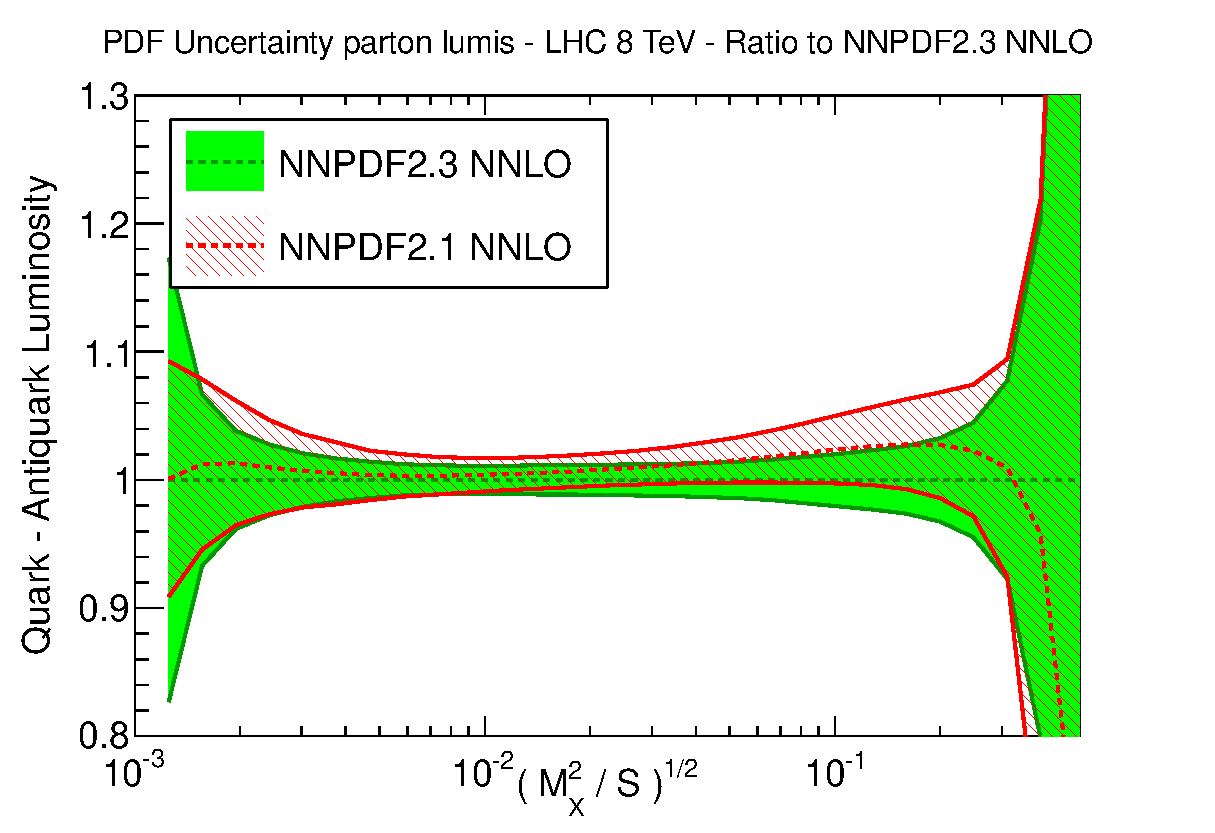
\includegraphics[width=0.50\textwidth]{qq_S_6_4e+07-rat-8tev}
    \end{center}
    \vskip-0.5cm
    \label{fig:pdf-jets}
\end{figure}

\vskip15pt
\center{Modest reduction in uncertainties on parton luminosities.}

\end{frame}

\begin{frame}
\frametitle{NNPDF2.3 vs NNPDF2.1 - strangeness}
\begin{itemize}
\item<1-> Isolate impact of LHC data upon strangeness - noLHC vs global
\end{itemize}

 \begin{figure}[b!]
    \begin{center}
         \includegraphics[width=0.50\textwidth]{pdf_xsplus_log_band_comparison.eps}
      \includegraphics[width=0.50\textwidth]{pdf_xsminus_log_band_comparison.eps}
    \end{center}
    \vskip-0.5cm
\end{figure}
\vskip15pt

\begin{itemize}
\item<1-> LHC data prefers a rather larger strange sea distribution at small-$x$.
\item<1->  Data insensitive to $s-\bar{s}$.
\end{itemize}

\end{frame}


\begin{frame}
\frametitle{Collider only PDFs with LHC data}
 \begin{figure}[b!]
    \begin{center}
      \includegraphics[width=0.50\textwidth]{pdf_xu_log_band_comparison.eps}
      \includegraphics[width=0.50\textwidth]{pdf_xd_log_band_comparison.eps} \\
      \includegraphics[width=0.50\textwidth]{pdf_xSigma_log_band_comparison.eps}
      \includegraphics[width=0.50\textwidth]{pdf_xg_log_band_comparison.eps}
    \end{center}
    \vskip-0.5cm
    \label{fig:pdf-jets}
\end{figure}

\end{frame}

\begin{frame}
\frametitle{Collider only PDFs with LHC data - strangeness}

\begin{itemize}
\item<1-> Substantial constraint upon strange sea distribution for the collider only fit.
\item<1->  Data once again insensitive to $s-\bar{s}$.
\end{itemize}

 \begin{figure}[b!]
    \begin{center}
          \includegraphics[width=0.50\textwidth]{pdf_xsplus_log_band_comparison_coll.eps}
      \includegraphics[width=0.50\textwidth]{pdf_xsminus_log_band_comparison_coll.eps}
    \end{center}
    \vskip-0.5cm
    \label{fig:pdf-jets}
\end{figure}

\begin{itemize}
\item<1-> Clear preference again for a larger strange distribution at small-$x$
\item<1->  Uncertainties still large w.r.t global fit
\end{itemize}

\end{frame}

\begin{frame}
\frametitle{Consistency Checks - $\chi^2$}

\begin{columns}
  \begin{column}{0.4\textwidth}
\small
 \begin{itemize}
\item<1-> Consider $\chi^2$ to each dataset in global fit, before and after inclusion of LHC data. \vskip20pt
\item<1-> Significant improvement in description of LHC data, without deterioration in fit quality to existing datasets.\vskip20pt
\item<1-> Demonstrates consistency of the global QCD analysis.

\end{itemize}
\end{column}

  \begin{column}{0.6\textwidth}

\begin{table}
\scriptsize
\begin{tabular}{|c||c|c||c|c|}
\hline 
& \multicolumn{2}{c||}{\bf NNPDF2.1} & \multicolumn{2}{|c|}{\bf NNPDF2.3}  \\
\hline 
\hline 
Experiment  & NLO & NNLO  & NLO  & NNLO  \\
\hline
Total  &   1.145&   1.162 &    1.101 &    1.139  \\  
 \hline 
NMC-pd              & $          0.97      $ & $          0.93      $  &  $          0.95      $  &  $          0.95      $    \\  
NMC                 & $          1.68      $ & $          1.58      $  &  $          1.61      $  &  $          1.59      $  \\  
SLAC                & $          1.34      $ & $          1.04      $  &  $          1.24      $  &  $          1.00      $   \\  
BCDMS               & $          1.21      $ & $          1.29      $  &  $          1.20      $  &  $          1.28      $    \\  
CHORUS              & $          1.10      $ & $          1.08      $  &  $          1.10      $  &  $          1.07      $    \\  
NTVDMN              & $          0.70      $ & $          0.50      $  &  $          0.43      $  &  $          0.56      $    \\  
 \hline
HERAI-AV            & $          1.04      $ & $          1.04      $  &  $          1.00      $  &  $          1.01      $   \\  
FLH108              & $          1.34      $ & $          1.23      $  &  $          1.29      $  &  $          1.20      $    \\  
ZEUS-H2             & $          1.21      $ & $          1.21      $  &  $          1.20      $  &  $          1.22      $    \\  
ZEUS $F_2^c$        & $          0.75      $ & $          0.81      $  &  $          0.82      $  &  $          0.90      $    \\  
H1 $F_2^c$          & $          1.50      $ & $          1.44      $  &  $          1.59      $  &  $          1.53      $   \\  
 \hline
DYE605              & $          0.94      $ & $          1.08      $  &  $          0.86      $  &  $          1.04      $    \\  
DYE886              & $          1.42      $ & $          1.69      $  &  $          1.27      $  &  $          1.58      $ \\  
 \hline
CDF $W$ asy         & $          1.88      $ & $          1.63      $  &  $          1.57      $  &  $          1.64      $   \\  
CDF $Z$ rap         & $          1.77      $ & $          2.38      $  &  $          1.80      $  &  $          2.03      $    \\  
D0 $Z$ rap          & $          0.57      $ & $          0.67      $  &  $          0.56      $  &  $          0.61      $   \\  
\textbf{ATLAS W,Z}         & $  \left[     1.57 \right]  $ & $  \left[     2.21 \right]   $  &  $          1.26      $  &  $          1.43      $   \\  
\textbf{CMS W el asy}      & $  \left[     2.02 \right]   $ & $  \left[     1.27 \right]   $  &  $          0.82      $  &  $          0.81      $    \\  
\textbf{LHCb W}            & $  \left[    0.89 \right]   $ & $  \left[     1.13 \right]   $  &  $          0.67      $  &  $          0.83      $    \\  
 \hline
CDF RII $k_T$       & $          0.68      $ & $          0.65      $  &  $          0.60      $  &  $          0.68      $   \\  
D0 RII cone         & $          0.90      $ & $          0.98      $  &  $          0.84      $  &  $          0.94      $    \\  
\textbf{ATLAS jets}          & $  \left[     1.06 \right]   $ & $  \left[     0.95 \right]   $  &  $          1.00      $  &  $          0.94      $  \\

\hline
\end{tabular}
\end{table}
\end{column}
\end{columns}

\end{frame}

\begin{frame}
\frametitle{Consistency Checks - $P(\alpha)$}
 \begin{itemize}
\item<1-> \small (In)consistency of LHC data with existing dataset can be studied with $P(\alpha)$.
\end{itemize}


%\begin{table}
%\begin{tabular}{c||c|c||c|c}
%\hline
%\multicolumn{5}{c}{NNPDF2.3 noLHC reweighted with LHC data}  \\
%\hline 
%\hline 
% & \multicolumn{2}{c||}{NLO} & 
%\multicolumn{2}{c}{NNLO} \\
%\hline 
%& $N_{\rm eff}$ & $\left< \alpha \right>$ & $N_{\rm eff}$ & $\left< \alpha \right>$ \\
%ATLAS W/Z & 285  & 1.4 & 134 & 1.6 \\
%CMS W e asy & 284 & 1.6  & 290  & 1.6 \\
%LHCb W & 492 & 1.1 & 483 & 1.2 \\
%ATLAS inclusive jets & 476  &  1.0 & 456  & 0.9 \\
%\hline
%All LHC data & 338 & 1.1 & 271 & 1.2 \\
%\hline 
%\end{tabular}
%\end{table}
%%%%%%%%%%%%%%%%%%%%%%%%%%%%%%
%
%
%%%%%%%%%%%%%%%%%%%%%%%%%%%%%%%%%%%%%%%%%%%%%%%%%
\begin{figure}
    \begin{center}
      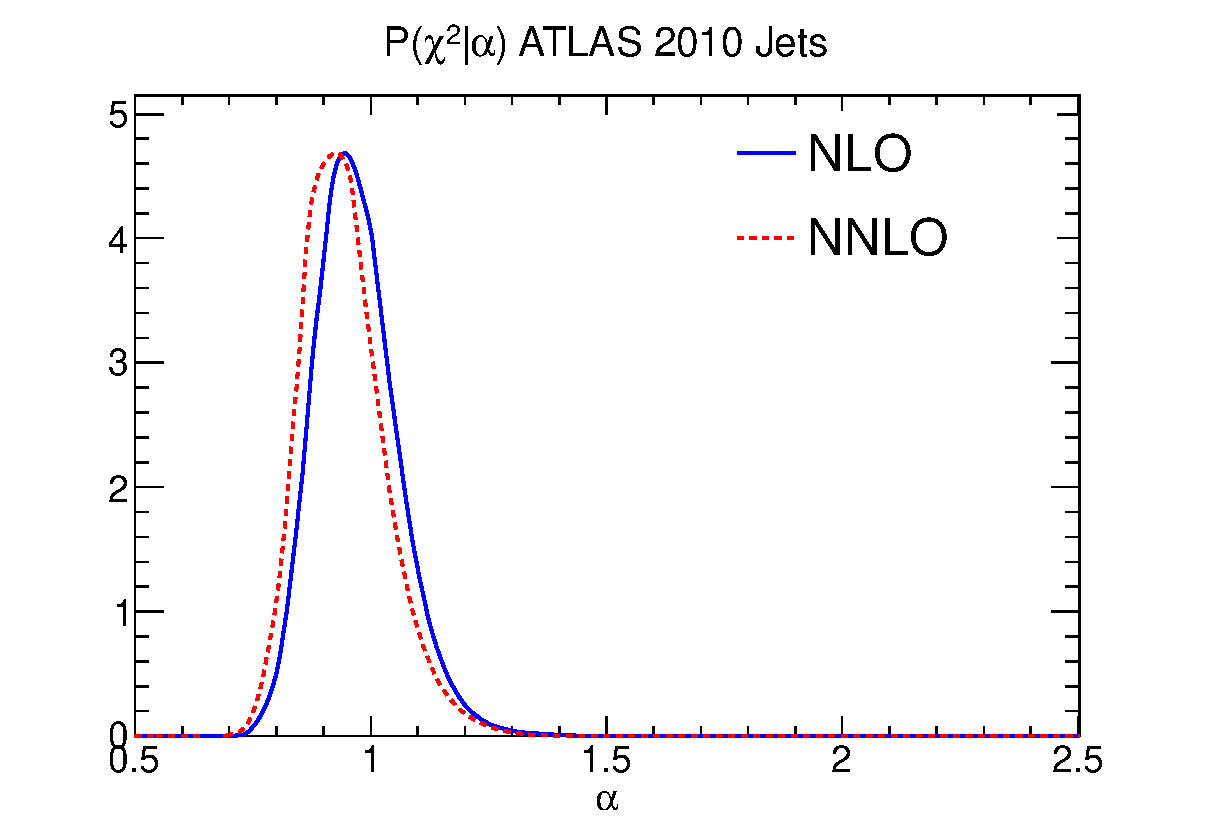
\includegraphics[width=0.4\textwidth]{palpha-atlasjets.eps}
      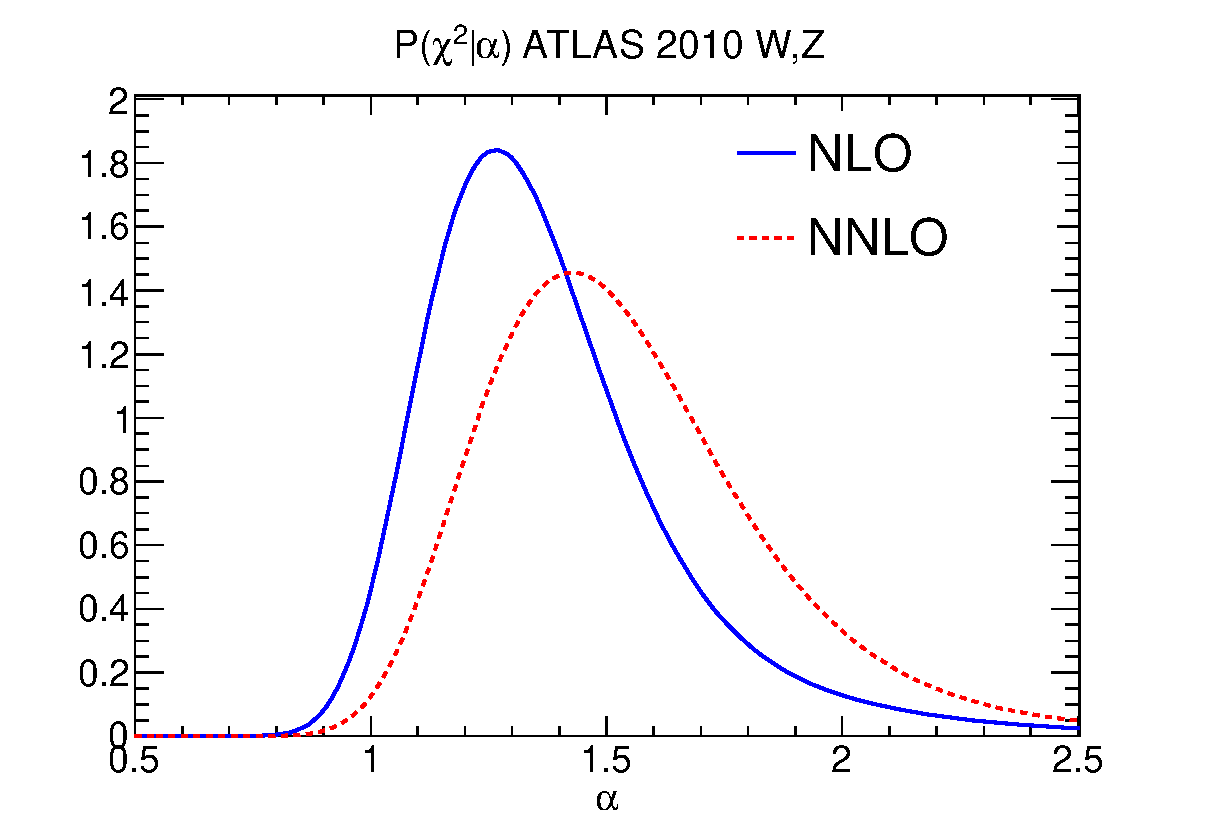
\includegraphics[width=0.4\textwidth]{palpha-atlaswz.eps}\\
      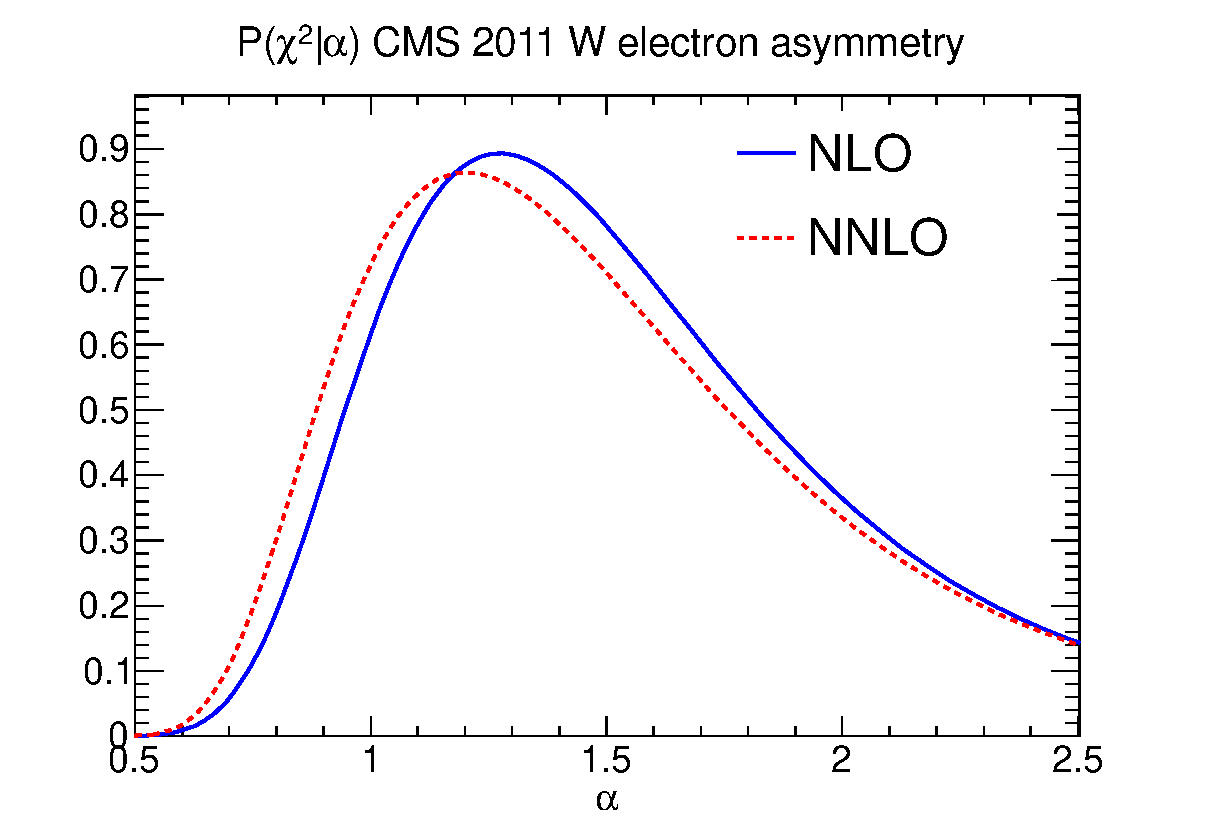
\includegraphics[width=0.4\textwidth]{palpha-cmswasy.eps}
      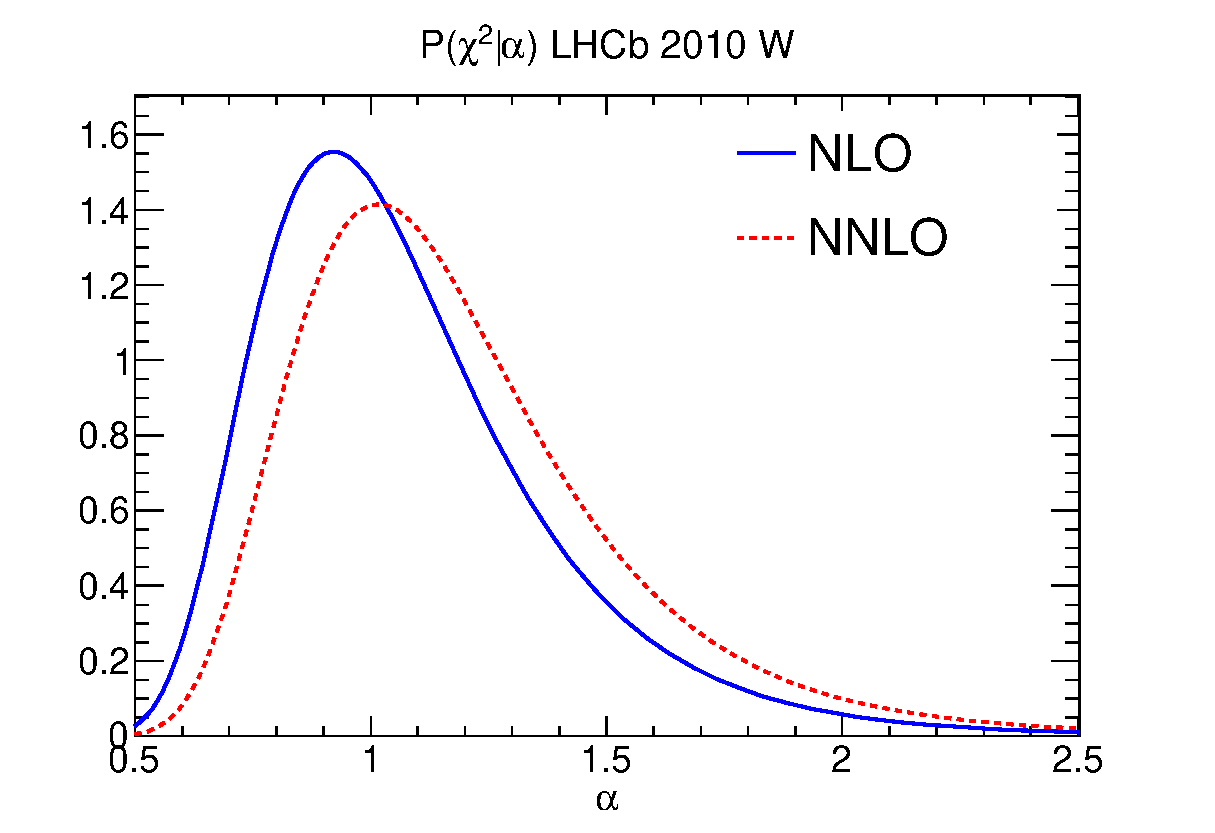
\includegraphics[width=0.4\textwidth]{palpha-lhcb.eps}
    \end{center}
\end{figure}

\end{frame}


\begin{frame}
\frametitle{Should we be using collider only PDFs yet?}

\begin{itemize}
\item<1-> LHC data providing excellent constraints upon previous collider only determination.
\end{itemize}

 \begin{figure}[b!]
    \begin{center}
      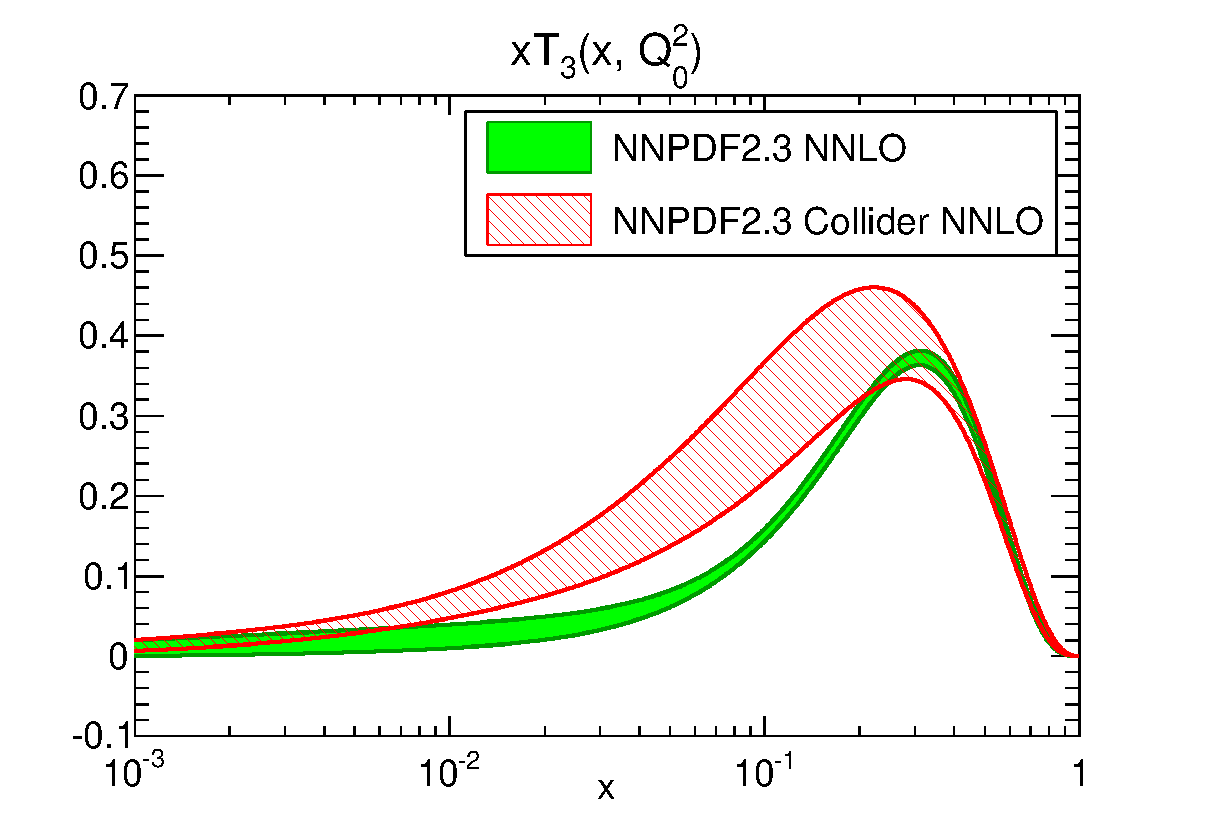
\includegraphics[width=0.50\textwidth]{xT3_Q_2_log-23-vs-23coll-nnlo.eps}
      \includegraphics[width=0.50\textwidth]{xSinglet_Q_2_log-23-vs-23coll-nnlo}
    \end{center}
    \vskip-0.5cm
    \label{fig:pdf-jets}
\end{figure}
\vskip10pt

\begin{itemize}
\item<1-> Collider only uncertainties remain large for flavour separation, strangeness.
\item<1-> Low energy data remains vital:
\begin{itemize}
\item<1-> NNPDF2.3 global fit is the recommended PDF set for precise phenomenology.
\end{itemize}

\end{itemize}

\end{frame}

\begin{frame}
\frametitle{Summary}

\underline{NNPDF Methodology and Reweighting} \vskip5pt
\begin{itemize} \small
\item<1-> NNPDF methodology provides a PDF determination free of parameterization bias, and with a robust propagation of experimental uncertainty.
\item<1-> Reweighting MC parton distributions can provide valuable insight into constraints offered by LHC data, regardless of the availability of a fast observable code.
\end{itemize}
\vskip20pt
\underline{NNPDF2.3} \vskip5pt
\begin{itemize} \small
\item<1-> New NNPDF parton set including constraints from LHC measurements of W/Z production and inclusive jet data.
\item<1-> Addition of LHC data to the fit enabled by the FK method for collider observables $\to$ extremely fast observable computation.
\item<1-> Strong constraints upon NNPDF collider only determination, however uncertainties remain large.
\end{itemize}
\end{frame}


\begin{frame}
    \begin{center}
      BACKUPS
    \end{center}
\end{frame}

\begin{frame}
\frametitle{NNPDF2.1 vs NNPDF2.3noLHC  -  strangeness}
 \begin{itemize}
 \item<1-> Corrected NuTeV dimuon cross section
 \end{itemize}
 
 \begin{figure}[b!]
    \begin{center}
      \includegraphics[width=0.50\textwidth]{xsp_Q_2_log-21-vs-23noLHC-nnlo.eps}
      \includegraphics[width=0.50\textwidth]{xsp_Q_2_log-21-vs-23noLHC.eps}
    \end{center}
    \vskip-0.5cm
\end{figure}
 
 
 \end{frame}

\begin{frame}
\frametitle{Unweighting procedure}
\begin{columns}
  \begin{column}{0.5\textwidth}
\begin{figure}
  \epsfig{width=0.7\textwidth,figure=unwplot-1.eps,angle=-90}\\
\end{figure}
  \end{column}
  \begin{column}{0.5\textwidth}
\begin{figure}
  \epsfig{width=0.7\textwidth,figure=unwplot-2.eps,angle=-90}
\end{figure}
  \end{column}
\end{columns}
\end{frame}


% End of slides
\end{document} 